\clearpage
\phantomsection
\addcontentsline{toc}{section}{Introduction}

\section*{Introduction}

\hspace*{2.5em} The Theory of Generalized Nets (GNs) provides a powerful mathematical apparatus for modeling and simulating complex processes characterized by parallelism and logical interdependence. Since its inception, the GN apparatus has established itself as a flexible tool in areas such as industrial production, computer systems, and artificial intelligence. However, with the growing complexity of models, the need for accessible and highly efficient software solutions for their description and study has become increasingly evident.

Despite the existing developments, there is still a lack of tools that enable work in an online environment, automatic generation of graphical representations, and straightforward integration into scientific publications. The main goal of the present work is the creation of the software system \textbf{\textit{OnlineGN}} -- a web-based simulator that combines the theoretical foundations of GNs with modern web technologies. Within the dissertation, new algorithms for automatic visualization and export of models are proposed, turning \textbf{\textit{OnlineGN}} into a comprehensive modeling environment. Through a series of simulations of classical problems and real manufacturing scenarios, the applicability and effectiveness of the developed tool are demonstrated.

\addtocontents{toc}{\vspace{-1.0em}}
\mysection{Generalized Nets: Theoretical Foundations and Simulation Software}


\subsection{Notes on the Theory of Generalized Nets}
\subsubsection{On the Concept of a Generalized Net}

\hspace*{2.5em}
Generalized Nets (GNs) were first presented in 1982 in a report at an international conference, with the text published in 1984 \cite{DIS-XY20}. They emerged as a natural continuation of efforts to model parallel processes, which began with the research of \textit{C.~A.~Petri} in 1962 and led to the formulation of Petri nets (PNs) \cite{DIS-XY1}.

In their classical form, PNs are bipartite directed graphs with two types of vertices: \emph{transitions} (discrete events) and \emph{places} (conditions), between which \emph{tokens} move. The orientation toward parallelism led to numerous extensions of PNs (more than twenty by 1982), which add: (i) temporal aspects; (ii) coloring of tokens for distinguishability; (iii) guard conditions (predicates) over groups of tokens for synchronized firings; and others.

Against this background, GNs provide a richer framework for the specification of concurrency, synchronization, and conditional dependencies, while preserving the intuitive graph semantics of PNs and extending their expressive power for modeling complex parallel processes. Detailed studies of GNs are given in \cite{DIS-Z3,DIS-Z1,DIS-BAM, DIS-AtanassovSotirova2017}, while a small part of their applications is considered in \cite{DIS-Orozova2011,DIS-Georgiev1998,DIS-StefanovaPavlova2001,DIS-Aladjov2002}.

\subsubsection{Informal Description of the Notation in Generalized Nets}

\hspace*{2.5em}In the dissertation, the main notation and rules in GNs are summarized. Places and transitions are connected by \textit{arcs}\ (arrows), which determine the possible directions of movement. Some places contain \textit{tokens}\ (dots), analogously to classical Petri nets~\cite{DIS-Q148}. An entering token carries \textit{initial characteristics}, and when passing through the net it may acquire additional characteristics. Since the initial characteristics may remain valid, a \textit{history} accumulates for the token. From the point of view of implementation, this set of characteristics can be regarded as an associative list ``name~$\to$~value''. A place may optionally have a \it characteristic function\rm, which assigns new values to the characteristics of the tokens entering it.

The connectivity in GNs is simplified with respect to degrees: each place is connected to at least one arc and may have at most one incoming and one outgoing arc. Without an incoming arc, a place is \it input\rm, and without an outgoing arc -- \it output\rm. Each transition has at least one input and one output place ($m, n \ge 1$); it is possible that, for a given transition, the same place plays both roles \cite{DIS-Z1}. When a token reaches an input place of a transition, it becomes \emph{potentially active}; if the conditions for transfer to the output places are satisfied, the transition is \it active\rm.

The conditions associated with transitions are not described by a single predicate, but by an \textit{indexed matrix}\ (IM) -- a matrix of predicates that simultaneously specifies when movement along the different directions is possible and determines the capacities of the corresponding arcs. Thus, the IM provides finer control in comparison with standard Petri nets \cite{DIS-Z1}.

Time in the definition of GNs is \textit{discrete}: successive steps are considered, numbered by an integer variable that increases by one. It is permissible to fix in parallel an \it absolute time scale\rm\ with an initial moment and a horizon of functioning \cite{DIS-Z1}. For multiple connected processes, separate scales may be used for each of them, or a common one for synchronization.

GNs are sufficiently expressive to describe both the extensions of Petri nets and models with the computational power of a Turing machine class (in particular, finite automata) \cite{DIS-Z1}. The GN extensions known so far are \it conservative\rm: for each of them there exists a standard GN that equivalently describes its functioning and result \cite{DIS-Z1, DIS-BAM}.

\subsubsection{Formal Definition of Generalized Nets}

\hspace*{2.5em}In this section, the dissertation considers a strictly mathematical definition of the GN components. The formal apparatus is based on set theory and the apparatus of IMs, defining the structure, temporal parameters, and token dynamics. Formally, each transition is described by the ordered 7-tuple
$$ Z = \langle L', L'', t_{1}, t_{2}, r, M, \kv \rangle, $$
where $r$ is the IM that specifies the transition conditions, and $M$ is the IM that specifies the capacities of the arcs of the transition; the transition is activated at moment $t_1$, provided that the truth value of the Boolean expression is ``true''. The generalized net is given by the ordered 4-tuple
$$ E = \langle \langle A, \pi_{A}, \pi_{L}, c, f, \theta_{1}, \theta_{2} \rangle,
\langle K, \pi_{K}, \theta_{K} \rangle, \langle T, t^{0}, t^{*} \rangle,
\langle X, \Phi, b \rangle \rangle, $$
where the transitions and places, priorities, capacities, time and memory functions, and characteristic functions are defined. The GN components are classified according to the static structure, dynamic nature, temporal essence, and memory of the GN, and the notion of an \textit{empty GN} is introduced.

\subsubsection[Algorithms for Token Movement in a Transition and in a Generalized Net]{Algorithms for Token Movement in a Transition and in a Generalized Net}\label{tokenMove}

\hspace*{2.5em}In this section, the dissertation presents an extended version of the most general algorithm known so far for the functioning of a transition in a GN \cite{DIS-Z1, DIS-Z3, DIS-BAM, DIS-AtanassovSotirova2017}.

\subsection{Current Software for Simulation of Generalized Nets}

\subsubsection{Main Shortcomings of Current Simulators}

\hspace*{2.5em}This section of the dissertation considers the main shortcomings of current simulators, which simultaneously affect architecture, user experience, and maintenance. These include \textbf{fragmentation and incomplete integration}, \textbf{portability and dependency problems}, as well as \textbf{language layer and compatibility}. These and other reasons motivate the development of \textit{OnlineGN} as a web-based, integrated, and platform-independent environment.

\subsubsection{Analysis of Existing Software Solutions}

\hspace*{2.5em}Existing software solutions for modeling and simulation of GNs are considered, describing the architecture, components, and interaction modes in \textbf{\textit{GN Lite}} (incl. \textit{GNTicker}, \textit{TickerServer/GNTP}, \textit{GN IDE}, \textit{GNVis}, \textit{XGN2SVG}, \textit{GNProfy}, \textit{GNDraw}), as well as the approach of \textbf{\textit{GoGN}} for developing models by means of a \textit{C\#} library. The emphasis is on the technologies used, the degree of integration between the tools, and the practical aspects of working with the \textit{XGN} format.

\subsubsection{Main Shortcomings of Current Simulators}

\hspace*{2.5em}The main shortcomings of current simulators are summarized below, as they affect architecture, user experience, and maintenance simultaneously.

\begin{itemize}
	\item \textbf{Fragmentation and incomplete integration.}\\
	Early versions of \textit{GNTicker} are console-based, while interactivity is compensated through \textit{TickerServer}/\textit{GNTP} and separate auxiliary tools outside the main modeling--simulation cycle.
	\item \textbf{Portability and dependency problems.}\\
	Some of the tools are aimed at \textit{Windows/.NET}, and under \textit{Unix}-like operating systems they often rely on \textit{Mono}, which increases installation and maintenance effort.
	\item \textbf{Language layer and compatibility.}\\
	\textit{GNTCFL} increases the learning curve; \textit{GNJS} aims to reduce it, but the prototypes do not provide full compatibility with \textit{GNTP}, which limits integration.
	\item \textbf{Scalability and performance.}\\
	The algorithms are correct, but not always optimal for very large or highly connected nets, which leads to longer execution times and higher resource consumption.
	\item \textbf{Limitations of the tooling and ecosystem.}\\
	\textit{XGN2SVG} produces static output; \textit{GNVis} is a separate \textit{.NET} module; \textit{GNProfy} is focused on sequence diagrams and older \textit{XMI} versions; \textit{GoGN} requires programming and compilation instead of declarative modeling.
\end{itemize}
\subsection{Aim and Tasks of the Dissertation}

\subsubsection{Formulation of the Aim}
\hspace*{2.5em}The aim of the present dissertation is to develop a web-based simulator for GNs -- \textit{OnlineGN}, which provides an interactive environment for creating, visualizing, editing, sharing, and simulating models, and to validate its applicability by developing, simulating, and verifying real GN models.

\subsubsection{Tasks for Achieving the Aim}
\hspace*{2.5em}To achieve the stated aim, the following tasks have been formulated:

\vspace{-0.2cm}

\begin{enumerate}[
	label=\textbf{Task \arabic*.},
	ref=Task \arabic*,            
	leftmargin=2.5em,
	labelsep=0.8em,
	align=left
	]
	\item Development and implementation of an algorithm for automatic drawing of GNs from their description in a structured textual format.
	\label{task:auto-draw}
	
	\item Development and implementation of an algorithm for converting an \textit{SVG} image of a GN into \textit{TeX} format, for easy inclusion of visualizations in scientific publications.
	\label{task:svg-to-tex}
	
	\item Formulation of requirements for a web-based solution.
	\label{task:requirements}
	
	\item Design of the architecture of the \textit{OnlineGN} system and definition of the main modules (net storage, visualization, editing, simulation, import/export, \textit{API}).
	\label{task:architecture}
	
	\item Implementation of a web-based graphical interface for visualization, editing, and personalization of the generated image (places, transitions, connections, and visual parameters).
	\label{task:web-ui}
	
	\item Implementation of a convenient interface for editing predicates in the indexed matrix and the characteristic functions of the places.
	\label{task:predicates-ui}
	
	\item Implementation of a mechanism for online storage and sharing of nets via a unique hyperlink (link), based on centralized database storage.
	\label{task:share-storage}
	
	\item Creation and formalization of new GN models of real processes that have not so far been described by means of GNs.
	\label{task:new-models}
	
	\item Simulation and verification of the developed models in \textit{OnlineGN} through scenarios and experiments.
	\label{task:simulation}
\end{enumerate}

The realization of the stated tasks will lead to the creation of a functional web-based simulator, accompanied by new algorithms for automatic drawing and conversion to \textit{TeX}. The practical applicability of the development will be confirmed by validation examples and by the formalization of new GN models of real processes.

\vspace{0.5cm}

In summary, the dissertation addresses the need for automation and effective collaboration when working with the GN apparatus. The \textit{OnlineGN} project offers a complete, flexible, and easy-to-use solution, aligned with contemporary software standards and the needs of the research community.

\mysection{Newly Introduced Algorithms for Generalized Nets}


\subsection{Algorithm for Automatic Drawing of Generalized Nets}
\label{sec:auto-drawing}

\hspace*{2.5em}The chapter presents the solution of \textbf{\ref{task:auto-draw}} through the development of an algorithm for automatic drawing of GNs, described in detail in \cite{DIS-DimitrievTerziev}.

\subsubsection{Introduction}
\hspace*{2.5em}When working with GNs, a significant difficulty is the need for substantial manual effort in drawing them. Traditionally, the coordinates of the elements are specified precisely, which is time-consuming and carries a risk of human error. The same problem is also observed in GN simulators, where manual input of coordinates slows down modeling and limits rapid experimentation.

In response, an algorithm for automated drawing is proposed, which generates clear visual representations of GNs solely from their abstract description and eliminates the need for manual specification of coordinates. In this way, the creation and manipulation of GNs are facilitated, and attention is directed toward analysis rather than toward the technical details of rendering.

\subsubsection{Current Practices in the Visualization of Generalized Nets}

\hspace*{2.5em}The visualization of GNs requires precise positioning of places, transitions, and arcs for the sake of clarity and structural correctness. Traditionally, this is done interactively through manual specification of coordinates, following established conventions for arrangement and readability.

\paragraph{Directionality of arrows.}
\mbox{}\\
Arrows are usually oriented from left to right, with the outputs of the transitions drawn on the right. When feedback connections are needed, they are added in a way that does not disrupt the overall clarity.

\paragraph{Positioning of output places.}
\mbox{}\\
Output places are positioned immediately to the right of the corresponding transitions, which facilitates tracing the flow and the logic of the net.

\paragraph{Places with a dual role (input and output).}
\mbox{}\\
When a place is both an input and an output, it is positioned in the lower part of the transition, with the aim of producing a more orderly diagram and minimizing crossings.

\paragraph{Additional practices.}
\mbox{}\\
For better readability, uniform spacing, clear labels, color differentiation when needed, minimization of crossings, and consistent orientation of the net are applied.

Although these practices support clear visualization, manual specification of coordinates remains labor-intensive and error-prone, which motivates automated solutions. In the following parts, an algorithm for automatic drawing of GNs is presented, consistent with the established conventions and reducing both manual effort and the risk of errors.

\subsubsection{Drawing Graphs}

\hspace*{2.5em}The visualization of graphs aims at a clear presentation of structure through suitable placement of vertices and edges with minimal crossings \cite{DIS-Kamada1989}. For this purpose, \textit{Graphviz} is often used -- a tool for automatic generation of graph images from a \textit{DOT} description, with various layout algorithms (e.g. \textit{dot}, \textit{neato}) \cite{DIS-Ellson2004}.

\subsubsection{Modeling a Generalized Net as a Directed Graph}

\hspace*{2.5em}For the purposes of visualization and structural analysis, a GN can be represented as a directed graph in which \textbf{places} and \textbf{transitions} are regarded as \textbf{vertices}, while the \textbf{arcs} describe directed connections between them. An arc \(l \rightarrow Z\) is drawn when place \(l\) is an input to transition \(Z\), and an arc \(Z \rightarrow l\) when \(l\) is an output of \(Z\). In this way, the direction of the arcs reflects the flow of tokens in the net.

\paragraph{Example.}
\mbox{}\\
A GN is considered with places \(l_1, l_2, l_3, l_4, l_5\) and transitions \(Z_1, Z_2, Z_3\), where the connections are:
\(l_1 \rightarrow Z_1\), \(Z_1 \rightarrow l_2, l_3\), \(l_2 \rightarrow Z_2\), \(Z_2 \rightarrow l_4\), \(l_3, l_4 \rightarrow Z_3\), \(Z_3 \rightarrow l_5\).
The GN is shown in \textbf{Figure~\ref{DIS-fig:gen-net-z1-z3}}, and the corresponding directed graph -- in \textbf{Figure~\ref{DIS-fig:gen-network-graph}}.

\begin{figure}[H]
	\centering
	\tiny
	\begin{center}
		\setlength{\unitlength}{14pt}
		\begin{picture}(18.47,7.73)
			\linethickness{0.4pt}
			% --- Transitions ---
			\put(3.05,7.98){\makebox(0,0)[b]{$Z_1$}}
			\put(3.05,6.67){\makebox(0,0)[bb]{\Large$\bigtriangledown$}}
			\put(3.05,6.67){\line(0,-1){6.67}}
			\put(9.27,7.98){\makebox(0,0)[b]{$Z_2$}}
			\put(9.29,6.67){\makebox(0,0)[bb]{\Large$\bigtriangledown$}}
			\put(9.29,6.67){\line(0,-1){3.33}}
			\put(15.40,7.98){\makebox(0,0)[b]{$Z_3$}}
			\put(15.42,6.67){\makebox(0,0)[bb]{\Large$\bigtriangledown$}}
			\put(15.42,6.67){\line(0,-1){6.67}}
			% --- Places ---
			\put(6.19,5.36){\makebox(0,0)[cc]{$l_2$}}
			\put(6.19,4.47){\circle{1.0}}
			\put(6.19,2.69){\makebox(0,0)[cc]{$l_3$}}
			\put(6.19,1.80){\circle{1.0}}
			\put(12.40,5.36){\makebox(0,0)[cc]{$l_4$}}
			\put(12.40,4.47){\circle{1.0}}
			\put(18.47,2.69){\makebox(0,0)[cc]{$l_5$}}
			\put(18.47,1.80){\circle{1.0}}
			\put(0.00,5.36){\makebox(0,0)[cc]{$l_1$}}
			\put(0.00,4.47){\circle{1.0}}
			% --- Edges ---
			% Z1 -> l2
			\put(3.07,4.47){\vector(1,0){2.62}}
			% Z1 -> l3
			\put(3.07,1.80){\vector(1,0){2.62}}
			% Z2 -> l4
			\put(9.31,4.47){\vector(1,0){2.59}}
			% Z3 -> l5
			\put(15.45,1.80){\vector(1,0){2.52}}
			% l1 -> Z1
			\put(0.50,4.47){\vector(1,0){2.52}}
			% l2 -> Z2
			\put(6.69,4.47){\vector(1,0){2.58}}
			% l3 -> Z3
			\put(6.69,1.80){\vector(1,0){8.71}}
			% l4 -> Z3
			\put(12.90,4.47){\vector(1,0){2.50}}
		\end{picture}
	\end{center}
	\normalsize
		\caption*{\textbf{Figure~\ref{DIS-fig:gen-net-z1-z3}} -- A generalized net with places $l_1, l_2, l_3, l_4, l_5$ and transitions $Z_1, Z_2, Z_3$.}
\end{figure}


\begin{figure}[H]
	\centering
	\begin{varwidth}{\textwidth}
		\centering
		\begin{tikzpicture}[
			node distance=0.4cm and 0.8cm,
			every node/.style={draw, shape=ellipse, minimum height=0.4cm, minimum width=0.8cm},
			->, >=Stealth
			]
			
			% Nodes
			\node (l1) {$l_1$};
			\node[right=of l1] (Z1) {$Z_1$};
			\node[above right=of Z1] (l2) {$l_2$};
			\node[right=of l2] (Z2) {$Z_2$};
			\node[right=of Z2] (l4) {$l_4$};
			\node[below right=of Z1] (l3) {$l_3$};
			\node[below right=of l4] (Z3) {$Z_3$};
			\node[right=of Z3] (l5) {$l_5$};
			
			% Arrows
			\draw (l1) -- (Z1);
			\draw (Z1) -- (l2);
			\draw (l2) -- (Z2);
			\draw (Z2) -- (l4);
			\draw (Z1) -- (l3);
			\draw (l4) -- (Z3);
			\draw (l3) -- (Z3);
			\draw (Z3) -- (l5);
		\end{tikzpicture}
		\captionsetup{width=0.6\linewidth, justification=centering}
		\caption*{\textbf{Figure~\ref{DIS-fig:gen-network-graph}} -- Directed graph corresponding to the GN. The vertices represent places and transitions, and the directed edges represent the flow between them}

	\end{varwidth}
\end{figure}

\subsubsection{Visualization of Generalized Nets with \textit{Graphviz}}

\hspace*{2.5em}For correct and readable visualization of GNs with \textit{Graphviz}, parameters and constraints are specified that preserve the standard arrangement of the elements.

\paragraph{Setting global parameters.}
\mbox{}\\
\textit{rankdir=LR} is used for left-to-right orientation and \textit{splines=ortho} for orthogonal arcs, which preserves the grid-like appearance of GNs and facilitates tracing the flow.

\paragraph{Defining the vertices for transitions.}
\mbox{}\\
Transitions are modeled as rectangular vertices (\textit{shape=rect}) with a small fixed width, while the height is set according to the number of output places in order to reflect their connection with multiple outputs.

\paragraph{Grouping the output places with \textit{subgraph}.}
\mbox{}\\
The transition and its output places are grouped in a \textit{subgraph} (e.g. \textit{cluster}), using \textit{rank=same} to align the outputs and preserve their proximity to the transition during automatic arrangement.

\paragraph{Managing the input arcs through ``invisible'' vertices.}
\mbox{}\\
In order to obtain a single input point and for the inputs to ``enter'' from the left, auxiliary ``invisible'' vertices are added in front of the transition, to which the input places are connected, and then these vertices are connected to the transition itself, while their relative positioning is fixed through grouping.


\subsubsection{Algorithm for Generating \textit{Graphviz} Strings from Generalized Nets}

\hspace*{2.5em}This section describes the algorithmic logic for generating a \textit{Graphviz} string from a GN (\textit{GN}). The algorithm has been created for automating GN visualization and guarantees that the resulting graph follows predefined layout parameters. The main function, \textit{generateGraphvizString}, uses several helper functions, which are responsible for mapping transitions and places, generating invisible vertices, and creating the necessary arcs between the elements of the GN.

The structure of the pseudocode, summarizing the main steps and the logic of the algorithm, is defined as follows:

\paragraph{Generating invisible vertices.}
\mbox{}\\
The function \textit{genInvisNodes} generates invisible vertices used for alignment of the transitions in the graphical layout of the graph.

\begin{algorithm}[H]
	\caption{genInvisNodes(result, genNet, transition)}
	\begin{algorithmic}
		\For{each inputPlace in transition}
		\State \texttt{result $\gets$ result + "invis\_node\_"{} + transition.name + "\_"{} + indexOf(inputPlace) + "[shape = point, width = 0.01, height = 0.01]"{} + newLine}
		\EndFor
	\end{algorithmic}
\end{algorithm}

\paragraph{Connecting the invisible vertices to the transitions.}
\mbox{}\\
The function \textit{genEdgeBetweenInvisNodesAndTransition} generates arcs from the invisible vertices to the transitions, providing correct alignment and connectivity.

\begin{algorithm}[H]
	\caption{genEdgeBetweenInvisNodesAndTransition(result, genNet, transition)}
	\begin{algorithmic}
		\For{each inputPlace in transition}
		\State \texttt{result $\gets$ result + "invis\_node\_"{} + transition.name + "\_"{} + indexOf(inputPlace) + \detokenize{" -> "} +   transition.name + ":w"{} + newLine}
		\EndFor
	\end{algorithmic}
\end{algorithm}

\paragraph{Generating transitions.}
\mbox{}\\
The function \textit{genTransitionsString} generates the necessary configuration for each transition in the GN, including the invisible vertices and the connections among them.

\begin{algorithm}[H]
	\caption{genTransitionsString(genNet, result)}
	\begin{algorithmic}
		\For{each transition in genNet.transitions}
		\State \texttt{result $\gets$ result + "subgraph cluster\_"{} + transition.name + "\{"}
		\State \texttt{result $\gets$ result + "style=invis"}
		\State \texttt{result $\gets$ result + "subgraph cluster\_"{} + transition.name + "\_0"{} + "\{"}
		\State \texttt{result $\gets$ result + transition.name +
			"[shape=rect, height=max(count(outputPlaces), count(inputPlaces)), width = 0.005]"}
		\State \texttt{call genInvisNodes(result, genNet, transition)}
		\State \texttt{call genEdgeBetweenInvisNodesAndTransition(result, genNet, transition)}
		\State \texttt{call genOutgoingPlacesFromTransition(result, genNet, transition)}
		\State \texttt{call genOutgoingEdgesFromTransition(result, genNet, transition)}
		
		\texttt{result $\gets$ result + "\}"}
		\EndFor
	\end{algorithmic}
\end{algorithm}

\paragraph{Generating output places and arcs.}
\mbox{}\\
Two separate functions are responsible for generating the output places and the corresponding arcs. In this way, it is guaranteed that the arcs between transitions and places are created correctly.

\begin{algorithm}[H]
	\caption{genOutgoingPlacesFromTransition(genNet, result, transition)}
	\begin{algorithmic}
		\State \texttt{result $\gets$ result + "\{rank = same;"}
		\For{each outputPlace in transition}
		\State \texttt{result $\gets$ result + outputPlace.name + ";"}
		\EndFor
		\State \texttt{result $\gets$ result + "\}"}
	\end{algorithmic}
\end{algorithm}

\begin{algorithm}[H]
	\caption{genOutgoingEdgesFromTransition(genNet, result, transition)}
	\begin{algorithmic}
		\For{each outputPlace in transition}
		\State \texttt{result $\gets$ result + transition.name \detokenize{" -> "} outputPlace.name  }
		\EndFor
	\end{algorithmic}
\end{algorithm}

\paragraph{Generating outgoing arcs from the places.}
\mbox{}\\
Finally, the function \textit{genOutputEdgesFromPlaces} generates arcs connecting the places to the invisible vertices, thus ensuring the correct alignment of the transitions.

\begin{algorithm}[H]
	\caption{genOutputEdgesFromPlaces(genNet, result)}
	\begin{algorithmic}
		\For{each place in genNet}
		\State \texttt{invisNodeIndex $\gets$ first invisible node index for the transition}
		\State \texttt{result $\gets$ result + place.name + \detokenize{" -> "} + "invis\_node\_"{} + "transitionName"{} + "\_"{} + invisNodeIndex + "[arrowhead=none]"}
		\EndFor
	\end{algorithmic}
\end{algorithm}

\paragraph{Main function for generating a \textit{Graphviz} string.}
\mbox{}\\
The main function \textit{genGraphvizString} combines all previous functions, generating the full \textit{Graphviz} string representing the GN.

\begin{algorithm}[H]
	\caption{genGraphvizString(genNet)}
	\begin{algorithmic}
		\State \texttt{result $\gets$ "\ {digraph G} "}
		\State \texttt{result $\gets$ result + "rankdir=LR;"}
		\State \texttt{result $\gets$ result + "splines=ortho;"}
		\State \texttt{call genTransitionsString(result, genNet)}
		\State \texttt{call genOutputEdgesFromPlaces(result, genNet)}
		\State \texttt{result $\gets$ result + "\}"}
	\end{algorithmic}
\end{algorithm}

The result of applying the described algorithm for generating a \textit{Graphviz} string is shown in \textbf{Figure~\ref{DIS-fig:gen-network-Graphviz}}. The visualization reflects the automatically generated GN structure before subsequent graphical processing.


\begin{figure}[H]
	\centering
	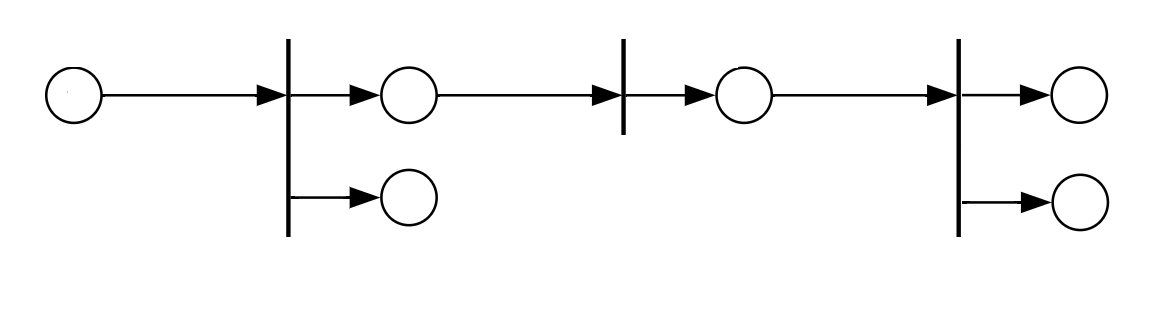
\includegraphics[width=\textwidth]{../../2. algos/drawing/images//genNetBeforePreprocess.png}
	\caption*{\textbf{Figure~\ref{DIS-fig:gen-network-Graphviz}} -- Example of a visualized graph (generalized net) using Graphviz.}
\end{figure}

\paragraph*{Subsequent processing of the generated image.}
\mbox{}\\
This paragraph describes the techniques applied to the \textit{SVG} (\textit{Scalable Vector Graphics}) file generated by the algorithm. Initially, a graph is created in which transitions are represented as very thin rectangular vertices and places -- as circular vertices. In order to adapt this visual representation to the GN form, a series of modifications is performed during subsequent processing.

The goal is for the resulting image to correspond more closely to the GN form. The specific changes are described below:

\begin{itemize}
	\item \textbf{Transitions:}  
	Each transition, initially defined as a narrow rectangle, is subjected to additional processing -- a black triangle is added in its upper part, which serves as a graphical identifier and improves its visibility in the overall structure. Above the triangle, a label with the name of the transition is visualized, guaranteeing its unambiguous identification in the model.
	
	\item \textbf{Places:}  
	For the places, represented by circles, their names are added above each circle. This is necessary because the tool for generating the initial \textit{SVG} (\textit{Graphviz}) does not support this way of labeling by default. Therefore, the required labels are inserted manually in order to ensure clarity in the final visual representation.
	
	
	\item \textbf{Visualization of the generalized net:}  
	After the application of the above changes, the resulting \textit{SVG} closely resembles a GN. The transitions are clearly marked and labeled, while the places have their names legibly placed above their circles. This approach leads to a more intuitive and accurate graphical representation of the system being modeled, facilitating its interpretation and analysis.
	
	The final result after applying the described steps for subsequent \textit{SVG} processing is shown in \textbf{Figure~\ref{DIS-fig:gen-network-processed}}. The resulting image follows the visual conventions of GNs and allows intuitive perception of structure and flow.
	
	
	\item \textbf{Example of the resulting image:}  
	\begin{figure}[H]
		\centering
		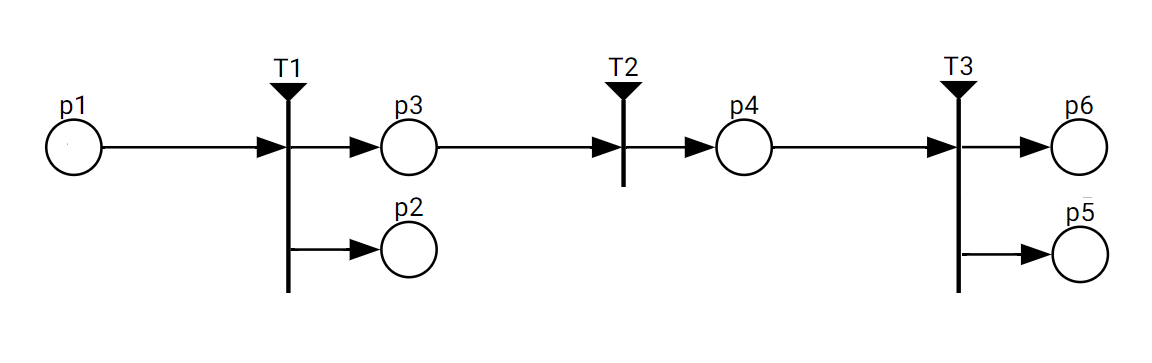
\includegraphics[width=\textwidth]{../../2. algos/drawing/images//genNetAfterPreprocess.png}
	\caption*{\textbf{Figure~\ref{DIS-fig:gen-network-processed}} -- Example of a generalized net after visualization processing.}
		
	\end{figure}
	
	\item \textbf{Pseudocode of the processing step:}
	
	\begin{algorithm}[H]
		\caption{postprocessSVG(graph)}
		\begin{algorithmic}
			\State \texttt{svg $\gets$ loadSVG(graph)}
			
			\For{each transition in svg}
			\State \texttt{points $\gets$ getTransitionPoints(transition)}
			\State \texttt{topPoint $\gets$ findTopMostPoint(points)}
			\State \texttt{addBlackTriangle(topPoint)}
			\State \texttt{label $\gets$ getTransitionLabel(transition)}
			\State \texttt{placeLabelAboveTriangle(topPoint, label)}
			\EndFor
			
			\For{each position in svg}
			\State \texttt{circle $\gets$ findCircle(position)}
			\State \texttt{centerPoint $\gets$ getCenterPoint(circle)}
			\State \texttt{label $\gets$ getPositionLabel(position)}
			\State \texttt{placeLabelAboveCircle(centerPoint, label)}
			\EndFor
			
			\State \texttt{outputSVG $\gets$ saveUpdatedSVG(svg)}
			\State \texttt{return outputSVG}
		\end{algorithmic}
	\end{algorithm}
	
	\item \textbf{Pseudocode of the main drawing function:}
	
	\begin{algorithm}[H]
		\caption{drawGenNet(genNet)}
		\begin{algorithmic}
			\State \texttt{graphvizStr $\gets$ genGraphvizString(genNet)}
			\State \texttt{svg $\gets$  Graphviz.render(graphvizStr)}
			\State \texttt{postprocessSVG(svg)}
		\end{algorithmic}
	\end{algorithm}
\end{itemize}

\subsection{Algorithm for Converting an \textit{SVG} Image of a Generalized Net into \textit{TeX} Format}

\hspace*{2.5em}This section presents an algorithm for automatic conversion of an \textit{SVG} image of a GN into \textit{TeX} code, thereby solving~\textbf{\ref{task:svg-to-tex}}.

\subsubsection{Introduction and Aim of the Algorithm}
\hspace*{2.5em}\textit{SVG} is a convenient vector format for generation and editing, but in scientific texts \textit{TeX} is most commonly used, where figures must fit cleanly and consistently with the style of the document. Therefore, a method is introduced for transferring an \textit{SVG} image of a GN into \textit{TeX} without manual redrawing.

The algorithm extracts places, transitions, and connections from the input \textit{SVG} and generates an equivalent diagram through \texttt{\textbackslash put}, \texttt{\textbackslash circle}, \texttt{\textbackslash line}, and \texttt{\textbackslash vector}. The resulting code is inserted directly into a document and minimizes the need for manual corrections.

\subsubsection{Description of the Format of the Input \textit{SVG} File}
\hspace*{2.5em}The algorithm works with an \textit{SVG} having a predefined structure. Each element has a \texttt{class} attribute indicating whether it is a place, a transition, or an arc. The GN components are represented as \texttt{<g>} groups:

\begin{itemize}
	\item \textbf{\textit{Places}}: \texttt{class} following the pattern \texttt{"node place \{id\}"}. Inside there are \texttt{<ellipse>} (visualization) and \texttt{<title>}, \texttt{<text>} (identifier).
	
	\item \textbf{\textit{Transitions}}: \texttt{class} following the pattern \texttt{"node transition \{id\}"}. The group contains two \texttt{<polygon>} elements (vertical line and triangle), marked with \texttt{class} \texttt{"triangle"}, as well as \texttt{<title>} and \texttt{<text>} for the identifier.
	
	\item \textbf{\textit{Edges}}: \texttt{class} following the pattern \texttt{"edge \{originId\}\_\_\{destinationId\}"}. The group contains a \texttt{<path>} (geometry of the arc) and a \texttt{<polygon>} (arrowhead).
\end{itemize}

\subsubsection{Extracting the Coordinates from the Input \textit{SVG} File}
\hspace*{2.5em}Only the coordinates required for construction in \textit{TeX} are parsed:

\begin{itemize}
	\item \textbf{\textit{Places}}: \texttt{cx, cy} from \texttt{<ellipse>} and \texttt{x, y} of the label from \texttt{<text>}.
	
	\item \textbf{\textit{Transitions}}: coordinates of the \textbf{two} \texttt{<polygon>} elements and \texttt{x, y} of the label from \texttt{<text>}.
	
	\item \textbf{\textit{Edges}}: from \texttt{<path>}, the \texttt{d} attribute is taken and parsed into a sequence of points \texttt{(x\_k,y\_k)} through the commands \texttt{M} and \texttt{L}. The arrowhead is parsed from \texttt{<polygon points="..."{}>} as points \texttt{(x\_j,y\_j)}.
\end{itemize}

Finally, the \textbf{global transformation} (e.g. \texttt{translate} and \texttt{scale}) is also extracted, and it is applied to all coordinates.

\subsubsection{Global Transformations and Normalization of Coordinates}
\hspace*{2.5em}The coordinates in \textit{SVG} are often subjected to a common transformation, which must be applied in order to obtain the correct scale and arrangement in \textit{TeX}. The typical format is:

\vspace{-0.3cm}

\begin{center}
	\texttt{transform="translate(tx, ty) scale(s)"}
\end{center}

\vspace{-0.2cm}

The following are extracted:
\[
\mathit{globalTranslate}_x = tx, \quad
\mathit{globalTranslate}_y = ty, \quad
\mathit{globalScale} = s
\]

\vspace{-0.2cm}

For each point \((x,y)\), the following is applied:

\vspace{-0.2cm}

\begin{equation}
	\widehat{X} = x \cdot s + tx, \quad
	\widehat{Y} = y \cdot s + ty
	\label{eq:svg-transform}
\end{equation}

After that, a common reduction factor is used:

\begin{equation}
	X' = \widehat{X} \cdot \underbrace{\tfrac{6}{10}}_{\text{LENGTH\_SCALE\_FACTOR}},\quad
	Y' = \widehat{Y} \cdot \underbrace{\tfrac{6}{10}}_{\text{LENGTH\_SCALE\_FACTOR}}
	\label{eq:svg-scale}
\end{equation}

Normalization to \texttt{picture} is needed because in \textit{TeX} the origin is at the bottom left, whereas in \textit{SVG} the \(y\)-axis grows downward, and because it is convenient for the coordinates to lie within the canvas. After computing the \textit{bounding box} \((X_{\min},X_{\max},Y_{\min},Y_{\max})\), each point is transformed as follows:

\vspace{-0.2cm}

\begin{equation}
	x_{\textit{TeX}} = (X' - X_{\min})\cdot c,\qquad
	y_{\textit{TeX}} = (Y_{\max} - Y')\cdot c
	\label{eq:tex-normalization}
\end{equation}

The dimensions of the canvas are set so as to fit the whole figure:

\vspace{-0.2cm}

\begin{equation}
	W = (X_{\max}-X_{\min})\cdot c,\qquad
	H = (Y_{\max}-Y_{\min})\cdot c
	\label{eq:picture-dimensions}
\end{equation}

\subsubsection{Normalization of Sizes and Labels}
\hspace*{2.5em}After normalization, sizes are unified and labels are corrected, since the scale and fonts in \textit{SVG/Graphviz} and \textit{TeX} differ.

\paragraph{Fixing the radius of the places.}
\mbox{}\\
The radius of the places is fixed through a constant circle diameter:
\begin{equation}
	\text{\texttt{\textbackslash circle\{1.0\}}} \quad \Rightarrow \quad r_{\textit{TeX}} = 0.5.
	\label{eq:fixed-place-radius}
\end{equation}

\paragraph{Correction of the labels of the places.}
\mbox{}\\
The label is shifted in the direction from the center toward its original position:
\begin{equation}
	L_{\textit{new}} = C + k\,(L-C),
	\label{eq:place-label-shift}
\end{equation}
where $k$ is \texttt{placeLabelOffsetFactor}.

\paragraph{Correction of the labels of the transitions.}
\mbox{}\\
The label of a transition is shifted upward by a constant:
\begin{equation}
	y_{\textit{new}} = y_{\textit{old}} - \texttt{transitionLabelVerticalOffset}.
	\label{eq:transition-label-offset}
\end{equation}

\subsubsection{Clipping the Arcs to the Boundaries of the Elements}
\hspace*{2.5em}In order for the arcs not to enter the places/transitions, the endpoints are clipped to the boundary of the corresponding element. The arc is \((p_0, p_1, \dots, p_{n-1})\), and only \(p_0\) (in the direction toward \(p_1\)) and \(p_{n-1}\) (in the direction away from \(p_{n-2}\)) are corrected.

\paragraph{Clipping the endpoints of arcs at places.}
\mbox{}\\
For a place (a circle with radius \(r_{\textit{TeX}}\)), the following is used:
\begin{equation}
	P' = C + r \cdot \frac{(P - C)}{\lVert P - C \rVert}.
	\label{eq:clip-circle}
\end{equation}

\paragraph{Clipping the endpoints of the arc at transitions.}
\mbox{}\\
The transition is approximated by a rectangle \([x_{\min},x_{\max}] \times [y_{\min},y_{\max}]\). The direction is determined from the adjacent point \(Q\) through:
\begin{equation}
	\Delta x = x_q - x_p,\qquad \Delta y = y_q - y_p.
	\label{eq:deltas}
\end{equation}
and the criterion:
\begin{equation}
	\text{horizontal, if } |\Delta x| \ge |\Delta y|,\qquad
	\text{vertical, if } |\Delta y| > |\Delta x|.
	\label{eq:dominant-dir}
\end{equation}
After that, the point is placed on the corresponding side:
\begin{equation}
	P'=
	\begin{cases}
		(x_{\max},\,y_p), & \text{if } |\Delta x|\ge|\Delta y| \text{ and } \Delta x>0,\\
		(x_{\min},\,y_p), & \text{if } |\Delta x|\ge|\Delta y| \text{ and } \Delta x<0,\\
		(x_p,\,y_{\max}), & \text{if } |\Delta y|>|\Delta x| \text{ and } \Delta y>0,\\
		(x_p,\,y_{\min}), & \text{if } |\Delta y|>|\Delta x| \text{ and } \Delta y<0.
	\end{cases}
	\label{eq:rect-clip}
\end{equation}

\paragraph{Preserving the correct endpoint of the arrowhead.}
\mbox{}\\
After clipping, the last segment is generated as \texttt{\textbackslash vector}, so that the arrowhead coincides with the new endpoint.

\subsubsection{Pseudocode of the Algorithm}

\noindent In a more general form, the steps can be synthesized as follows:
\begin{verbatim}
	function svgToTeX(svgString):
	1) DOM = parse SVG string into an XML DOM object
	2) mainG = find <g id="graph0"> and parse
	transform="translate(tx, ty) scale(s)"
	globalTranslate = (tx, ty)
	globalScale = s
	3) Define LENGTH_SCALE_FACTOR = 0.6   # (2/3) shrink
	4) Define pxToTeX = 0.1              # 1px -> 0.1 TeX units
	
	# 5) Identify PLACES
	for each g with class="node place":
	read ellipse(cx, cy)
	apply global transform + LENGTH_SCALE_FACTOR => (x', y')
	store nodeShapes[placeName] = circle with center=(x', y')
	and forced radius=5px
	
	# 6) Identify TRANSITIONS
	for each g with class="node transition":
	read polygon points => bounding box => xMin, xMax, yMin, yMax
	apply transform => store nodeShapes[transitionName] = rect
	
	# 7) Capture LABELS for places and transitions
	for each place:
	read original label coords => (lx, ly)
	apply transform => (lx', ly')
	offset label => (lx'', ly'') = (cx', cy')
	+ alpha*(lx'-cx', ly'-cy')
	for each transition:
	shift label upward => labelY' = labelY - someVerticalOffset
	
	# 8) Identify EDGES
	for each g with class="edge":
	read origin, destination from class or <title> text
	parse path (M x0 y0 L x1 y1 ...)
	apply transform => rawPoints
	# arrow polygon => transform as well
	
	# 9) CLIP edge endpoints
	for first and last rawPoints:
	if shapes[origin] == circle => move boundary
	if shapes[destination] == rect => clamp to bounding box
	(similarly for the other end)
	
	# 10) Compute bounding box over all x' and y'
	xMinAll, xMaxAll, yMinAll, yMaxAll
	
	# 11) Convert to TeX coords => (x_T, y_T)
	x_T = (x' - xMinAll)*pxToTeX
	y_T = (yMaxAll - y')*pxToTeX
	
	# 12) Build a \begin{picture}(width, height) with lines for edges,
		circles for places, etc.
		
		return final TeX code as a string
	\end{verbatim}
	
	\vspace{-0.45cm}
	
	After executing these steps, a \textit{TeX} fragment is generated that can be be directly inserted into a scientific document, in accordance with the accepted convention for drawing GNs.
	
	\mysection{\textit{OnlineGN}: Simulator for Generalized-Net Models}
	
	\hspace*{2.5em}The present chapter introduces the new GN simulator developed within the dissertation work -- \textit{OnlineGN}. The system requirements, architectural decisions, and the technology stack used are considered. The system is a standalone software component, and in future stages it is intended to expand compatibility through work with file formats generated by other simulators. The main functionalities are demonstrated in a video demonstration \cite{DIS-OnlineGN-video}. The source code of the application is published in \cite{phdThesisOnlineGNRepo}.
	
	\subsection{Requirements and Goals of the System}
	
	\hspace*{2.5em}The section defines functional and non-functional requirements for the web-based solution, which serve as criteria for the design and evaluation of \textit{OnlineGN}.
	
	\subsubsection{Functional Requirements}
	\hspace*{2.5em}\textit{OnlineGN} visualizes GNs in a two-dimensional space (places, transitions, and connections) and performs simulation by applying Algorithm B (see \textbf{\ref{tokenMove}}), while respecting the correct processing order of transitions/states/tokens and supporting changes of characteristics, token splitting, and token merging. Two execution modes are implemented: trace mode (step by step) and continuous execution until a final state (or a stopping criterion).
	
	The system allows restart of the simulation, interactive modification of coordinates of elements and connections (including points along a connection), as well as editing of characteristics of places and transitions with reflection in the simulation. Detailed information about the tokens at each step is provided, as well as a log of the operations within a single time step, describing the processing order according to priorities and capacities.
	
	Loading/saving of nets in \textit{JSON} format is supported, as well as storage and retrieval from a database, generation of a hyperlink for access to a stored net, generation of a representation in \textit{TeX} format, addition of user-defined \textit{JavaScript} functions, and dynamic change of the simulation speed. Automatic deletion of nets that have not been accessed for a predefined period is also implemented.
	
	\subsubsection{Non-Functional Requirements}
	\hspace*{2.5em}The non-functional requirements cover performance, reliability, security, usability, and scalability. Thresholds are defined for response time up to 2 seconds under light load and recovery time after failure up to 30 minutes, and the choice is justified with respect to established practices and criteria for responsiveness and availability \cite{DIS-Nielsen1993RT}. In addition, the system does not collect personal data and is aligned with the requirements of \textit{GDPR}.
	
	\subsubsection{Constraints and Assumptions of the Environment}
	\hspace*{2.5em}The system is deployed using the free cloud services of \textbf{\textit{Render}} (for the server) and \textbf{\textit{Atlas}} (for the database), and is therefore designed in accordance with the limited resources provided by these services.
	
	\subsection{Architecture of the System}
	
	\hspace*{2.5em}The section describes the architectural organization of \textit{OnlineGN} and the interaction between the main components, corresponding to the implementation of \textbf{\ref{task:architecture}}.
	
	\subsubsection{General Architecture and Interaction Scenarios}
	\hspace*{2.5em}\textit{OnlineGN} is implemented as a three-layer architecture: data layer (DB), server layer (\textit{API}/services), and client layer (user application), where the client carries out the main part of the business logic and the server provides auxiliary services. The database stores nets and states and is responsible for data consistency; the server acts as an intermediary between the client and the DB and performs supporting tasks (e.g. periodic deletion of outdated records); the client implements the \textit{UI/UX}, visualization, simulation, and interactive modifications.
	
	\hspace*{2.5em}Typical scenarios are described: loading a net from the DB and starting a simulation, storing a net with a returned hyperlink, as well as periodic deletion of unused nets by the server.
	
	\subsubsection{Physical/\textit{Deployment} Architecture and Cloud Infrastructure}
	\hspace*{2.5em}The deployment is implemented through \textbf{\textit{Render}} and \textbf{\textit{MongoDB Atlas}}. The server instance is maintained in the infrastructure of \textit{Render} and delivers the client application to the browser, while the client--server communication is over \textit{HTTPS}. The database instance is maintained in \textit{Atlas}; the server communicates with the DB over \textit{HTTPS} and authenticates with a username and password \cite{DIS-RenderWebServices,MongoDBAtlasDocs}.
	
	\subsubsection{Technology Stack and External Dependencies}
	\hspace*{2.5em}The database is \textit{MongoDB} (version 8.0), where the data are stored as documents with a \textit{JSON}-like structure and a physical representation in \textit{BSON}.
	
	The server side is implemented with \textit{Node.js} and \textit{Express.js} for a \textit{REST API}, with unified routing, validation, and centralized error handling. The used \textit{Node.js} version is 22.x (\textit{LTS}), selected because of its predictable life cycle and long-term security updates; the approach supports a low migration cost to the next \textit{LTS} version. For the server, external libraries such as \texttt{body-parser}, \texttt{cors}, \texttt{cron}, \texttt{express}, \texttt{is-svg}, and \texttt{mongoose} are used, and for development -- \texttt{nodemon}.
	
	The client application is developed with \textit{Angular} (version 16) on top of \textit{TypeScript} and \textit{SCSS}, following good practices for maintainability and future transition to the next \textit{LTS} version \cite{DIS-AngularDocs,DIS-TypeScriptHandbook}. In addition to the core \textit{Angular} packages, \textit{Angular Material} and \textit{CDK} are used for \textit{UI} components, \texttt{ngx-toastr} for notifications, as well as \texttt{d3} and \texttt{d3-graphviz} for interactive visualization, animations, and rendering of \textit{Graphviz DOT} in the browser \cite{DIS-D3Transition}.
	
	\subsection{Design and Modules of the Application}
	\hspace*{2.5em}In the context of \textbf{\ref{task:architecture}}, the modular organization of \textit{OnlineGN} is presented. The main functional components (storage, visualization, editing, simulation, import/export, and \textit{API}) and the interaction between them are described. The modular design aims at clear separation of responsibilities (\textit{separation of concerns}), facilitated maintenance, and scalability.
	
	\subsubsection{Data Processing Module (\textit{GenNet Persistence})}
	\hspace*{2.5em}\textit{GenNet Persistence} implements the persistence of net data and provides the basic operations for working with records. The following submodules are included:
	\begin{itemize}
		\item \textbf{\textit{Loading}} -- loading a net by unique identifier, while updating the information about last use upon access;
		\item \textbf{\textit{Saving}} -- storing/updating the data of a net so that it is available for subsequent retrieval;
		\item \textbf{\textit{Expiration}} -- automatic deletion of nets that have not been accessed in the last 90 days.
	\end{itemize}
	
	\subsubsection{\textit{JSON} Format for Description of Generalized Nets}
	\label{subsec:gn-json-format}
	
	\hspace*{2.5em}The dissertation describes a developed \textit{JSON} format for unified, machine-readable representation of GNs, suitable for direct interpretation by the simulator. The data format is defined by the \textit{GenNetExportModel} interface. A single document describes the structure of the net, the initial configuration of the tokens, execution parameters, user-defined functions, and a pre-generated visualization. The format is organized into four main sections: \texttt{genNetRaw}, \texttt{settings}, \texttt{code}, and \texttt{svg}.
	
	\paragraph{Root structure.}\mbox{}\\
	The root object contains:
	\begin{itemize}
		\item \texttt{\textbf{\textit{genNetRaw}}} -- declarative description of the GN;
		\item \texttt{\textbf{\textit{settings}}} -- settings of the simulation environment;
		\item \texttt{\textbf{\textit{code}}} -- user \textit{JavaScript} code;
		\item \texttt{\textbf{\textit{svg}}} -- pre-generated visualization of the net.
	\end{itemize}
	
	In this way, a clear distinction is ensured between structural data and behavioral specification.
	
	\paragraph{Section \texttt{genNetRaw}.}\mbox{}\\
	The \texttt{genNetRaw} section contains the main data for the net and includes the collections \texttt{places}, \texttt{transitions}, and \texttt{tokens}.
	
	\begin{itemize}
		\item \texttt{\textbf{\textit{places}}} -- an array of objects of type \textit{Place}, through which the identifier, name, transformation function of the characteristics, merge function, priority, and capacity of the place are specified;
		\item \texttt{\textbf{\textit{transitions}}} -- an array of objects of type \textit{Transition}, through which the identifier, name, split function, priority, and the connections between the input and output places through objects of type \textit{TransitionItem} are specified;
		\item \texttt{\textbf{\textit{tokens}}} -- an array of objects of type \textit{Token}, defining the initial configuration of the simulation through identifier, name, current place, priority, and initial characteristics.
	\end{itemize}
	
	The dissertation gives example \textit{JSON} representations of objects of type \textit{Place}, \textit{Transition}, and \textit{Token}.
	
	\paragraph{Section \textit{\texttt{settings}}.}\mbox{}\\
	The \texttt{settings} section contains parameters that influence execution without changing the structural model. In the considered implementation, the object \texttt{simulationSettings} is included, through which the duration of one simulation step is specified by means of \texttt{stepDurationMS}.
	
	\paragraph{Section \textit{\texttt{code}}.}\mbox{}\\
	The \texttt{code} section contains a string with user \textit{JavaScript} code used in the simulation. In order for the code to be accessible in the context of the simulator, the object \texttt{\textbf{\textit{this.globalObj}}} is defined at the outermost level, serving as a namespace for user definitions.
	
	\hspace*{2.5em}Within \texttt{\textbf{\textit{this.globalObj}}} there are:
	\begin{itemize}
		\item \texttt{\textbf{\textit{tokens}}} -- a reference to the current collection of tokens;
		\item \texttt{\textbf{\textit{functions}}} -- functions invoked by their names from the fields in \texttt{\textbf{\textit{genNetRaw}}};
		\item \texttt{\textbf{\textit{globals}}} -- additional values used as auxiliary context during execution of the simulation.
	\end{itemize}
	
	Thus, the format allows declarative specification of the net, while the concrete behavior and the conditions during the simulation are defined centrally and linked through the names of the functions. The dissertation also presents an example \textit{JSON} model of a GN with two places, one transition, and one token.
	
	\paragraph{Section \textit{\texttt{svg}}.}\mbox{}\\
	The \texttt{svg} section contains an \textit{SVG} string for visualization of the net. If such a string is not provided, the program generates an \textit{SVG} visualization through the automatic drawing algorithm described in \textbf{\ref{sec:auto-drawing}}.
	
	\subsubsection{Graphical Visualization Module (\textit{SVG/Graphviz})}
	\hspace*{2.5em}The module for GN visualization in the client application is discussed: loading a ready \textit{SVG} or generating an \textit{SVG} from a \textit{Graphviz} string, drawing/redrawing elements, animations upon changes, processing user events, and saving the current state as \textit{SVG}.
	
	\subsubsection{Simulation Module for the Movement of Tokens}
	\hspace*{2.5em}The \textit{Simulation} module is described, which implements execution of the simulation according to the rules of GNs and synchronizes the logical changes with the visualization: a single move (\textit{Single move}), full simulation (\textit{Full simulation}), and restart (\textit{Reset}) through a visualization update submodule (\textit{Update visualization}).
	
	\subsubsection{\textit{API} and Script Interface}\label{sec:api-script-interface}
	
	The server provides two endpoints for access from the client.
	
	\vspace{-10pt}
	\begin{itemize}
		\item \texttt{\textbf{\textit{GET /api/genNets/:id}}} -- retrieves a net by identifier and returns \texttt{\textbf{\textit{status code 200}}} on success or \texttt{\textbf{\textit{status code 404}}} if the net is not found
		\item when the net is found, an object with fields \texttt{\textbf{\textit{id}}}, \texttt{\textbf{\textit{content}}}, and \texttt{\textbf{\textit{lastFetchedAt}}} is returned
		\item \texttt{\textbf{\textit{POST /api/genNets}}} -- stores the submitted net in the database
		\item in the request, the field \texttt{\textbf{\textit{content}}} is submitted, and upon successful storage \texttt{\textbf{\textit{status code 201}}} and \texttt{\textbf{\textit{id}}} are returned
		\item upon unsuccessful storage, \texttt{\textbf{\textit{status code 400}}} is returned
	\end{itemize}
	
	At this point in the dissertation, example requests and \textit{JSON} responses from the \textit{API} are given.
	
	\subsubsection{Module for Importing and Exporting Nets}
	\hspace*{2.5em}The import and export module provides loading and saving of the net data in different formats, in accordance with the interface described in \textbf{item~\ref{sec:api-script-interface}}. Export to a \textit{JSON} file, \textit{TeX} format, and \textit{JSON} format in a database is supported, as well as import from a file and from stored \textit{JSON} data in the database. Functionally, the module is divided into two submodules: \textit{Import} (loading) and \textit{Export} (saving).
	
	\paragraph{Submodule \textit{Import}.}
	\mbox{}\\
	
	\vspace{-0.35cm}
	
	\textit{Import} includes:
	\vspace{-0.15cm}
	\begin{itemize}
		\item \textbf{\textit{JSON}} -- reading and validation of input data in \textit{JSON} format against the interface from \textbf{item~\ref{sec:api-script-interface}}, where upon successful validation the necessary objects for visualization are created; it is also used when loading from the server, since the data arrive in \textit{JSON};
		\item \textbf{\textit{File}} -- processing of files provided by the user, where for valid \textit{JSON} the content is passed to the \textit{JSON} submodule.
	\end{itemize}
	
	\paragraph{Submodule \textit{Export}.}
	\mbox{}\\
	
	\vspace{-0.35cm}
	
	\textit{Export} includes:
	\vspace{-0.15cm}
	\begin{itemize}
		\item \textbf{\textit{TeX}} -- conversion of the current visualization of the net into \textit{TeX} format for integration into scientific documents;
		\item \textbf{\textit{JSON}} -- generation of a \textit{JSON} representation of the currently loaded net (including data for tokens and visualization) according to the format from \textbf{item~\ref{sec:api-script-interface}}; it is also used when storing in the database;
		\item \textbf{\textit{File}} -- creation of a file for download by the user, where the data are generated by the \textit{JSON} submodule and written into a file.
	\end{itemize}
	
	\subsubsection{Module for Visualization of Dynamic Processes and Animation}
	\hspace*{2.5em}For visualization of token movement in the simulator, the \textit{d3} library is used, where each token is represented by an \textit{SVG} group (graphical symbol and text). The movement is implemented along trajectories defined by means of \textit{SVG path} elements, while the animation is executed through interpolation: the path length is computed (\texttt{getTotalLength()}), a transition is defined with \texttt{attrTween} and parameter $t\in[0,1]$, and the current position is obtained through \texttt{getPointAtLength(t * l)} and applied through the transformation \textit{translate}. After completion of the transition, the element is removed from the \textit{DOM}, which frees resources and reflects the traversal of the token along the arc.
	
	\subsection{Algorithms and Implementation Details}
	\hspace*{2.5em}The main algorithms and the key implementation decisions used in the realization of \textit{OnlineGN} are described.
	
	\subsubsection{Developed Algorithm 1: Automatic Drawing of GNs}
	\hspace*{2.5em}Algorithm~1 is implemented programmatically in the \textit{OnlineGN} system as a separate implementation, which automates GN drawing on the basis of the structural data of the net. The implementation generates coordinates and a graphical representation, which is used directly by the visualization module.
	
	\subsubsection{Developed Algorithm 2: Conversion of \textit{SVG} to \textit{TeX}}
	\hspace*{2.5em}Algorithm~2 is implemented in \textit{OnlineGN} for automatic conversion of the current \textit{SVG} visualization into a \textit{TeX} representation. The implementation transforms the main graphical primitives and textual elements, providing export in \textit{TeX} format for inclusion in scientific documents.
	
	\subsection{Interface and User Experience}
	
	\hspace*{2.5em}The chapter presents the implementation of \textbf{\ref{task:web-ui}} and \textbf{\ref{task:predicates-ui}}, considering the design of the user interface and the main principles of the user experience in \textit{OnlineGN}. The emphasis is on navigation, visual components, and the way in which the interface supports interactive work with the simulator, including visualization, personalization, and editing of GN parameters.
	
	\subsubsection{Navigation and Visual Components of the Web Client}
	
	\hspace*{2.5em}The client application combines the main functionalities in one primary workspace: visualization of the net, control of the simulation, and access to operations for loading/saving and exporting. The interface provides a direct view of the current state of the net and of the simulation step, as well as convenient access to the main actions through functional buttons and dialogs.
	
	\begin{figure}[H]
		\centering
		\setlength{\fboxrule}{2pt}
		\setlength{\fboxsep}{2pt}  
		\fbox{
\includegraphics[width=0.9\linewidth]{"../../3. onlineGn/images/ui-main-screen.png"}}
		\caption*{\textbf{Figure~\ref{DIS-fig:ui-main-screen} -- Main workspace and controls.}}
	\end{figure}
	
	For the implementation of \textbf{\ref{task:predicates-ui}}, an editing mode for the elements of the net has been introduced, through which a place/transition/arc is selected and its coordinates and parameters are modified. This enables interactive correction of the visualization and adjustment of the net objects directly in the workspace.
	
	\begin{figure}[H]
		\centering
		\setlength{\fboxrule}{2pt}
		\setlength{\fboxsep}{3pt}
		\fbox{
\includegraphics[width=0.85\linewidth]{"../../3. onlineGn/images/ui-edit-positions-mode.png"}}
		\caption*{\textbf{Figure~\ref{DIS-fig:ui-edit-positions-mode}} -- Coordinate editing mode (``Edit positions'').}
		
	\end{figure}
	
	\vspace{-0.3cm}
	
	Predicates and movement rules are visualized through specialized components for editing and viewing transitions, including a representation of the predicate matrix, which reflects the conditions for passage between the input and output places of a transition.
	
	\vspace{-0.3cm}
	
	\begin{figure}[H]
		\centering
		\setlength{\fboxrule}{2pt}
		\setlength{\fboxsep}{0pt}
		\fbox{
\includegraphics[width=0.5\linewidth]{"../../3. onlineGn/images/ui-transition-matrix.png"}}
		\caption*{\textbf{Figure~\ref{DIS-fig:ui-transition-matrix}} -- Predicate matrix of a specific transition.}
		
	\end{figure}
	
	\subsubsection{Help System, Documentation, and Localization}
	
	\hspace*{2.5em}A help system is provided, complementing the web client through embedded documentation and contextual help. Capabilities for interface localization are also ensured, which facilitates the use of the simulator in an educational and research context.
	
	\mysection{Applications of Generalized Nets and the \textit{OnlineGN} Simulator}
	\hspace*{2.5em}The present chapter considers four new GN models of processes that had not previously been described by means of the GN apparatus. Each of the developed models has been simulated and verified through the software environment \textit{OnlineGN}. The exposition and the simulations carried out in these four sections constitute the solution of \textbf{\ref{task:new-models}} and \textbf{\ref{task:simulation}}.
	
	\subsection{Simulation of Finite Automata through Generalized Nets}
	
	\hspace*{2.5em}The dissertation considers how a finite automaton can be described and simulated with the help of GNs. The correspondence between the states and transitions of the automaton and the corresponding GN elements is constructed so that the model becomes an operational scheme. A concrete example of a finite automaton is also considered, for which the corresponding GN is constructed and a real simulation is realized with \textit{OnlineGN}. In the development and analysis, the approach proposed in \cite{DIS-DimitrievAutomata} is followed.
	
	In \cite{DIS-Atanassov1985GNFA} a way of representing automata through GNs is considered, but the main emphasis is on the theoretical proof of existence; here, a construction directly applicable to simulation in GN software environments is given, with concrete structural constraints and optimizations.
	
	\subsubsection{Basic Notions of Finite Automata}
	
	\paragraph*{Finite alphabets and languages.}
	\mbox{}\\
	The standard notions of a \emph{finite alphabet} $\Sigma$, a \emph{word} $\alpha \in \Sigma^*$, and a \emph{language} $L \subseteq \Sigma^*$ are used, where the empty word is denoted by $\varepsilon$.
	
	\paragraph*{Deterministic Finite Automaton (DFA).}
	\mbox{}\\
	A DFA is a 5-tuple $\mathcal{A}=(Q,\Sigma,\delta,q_{\textit{start}},F)$ \cite{DIS-HopcroftMotwaniUllman,DIS-Kozen}, where $\delta:Q\times\Sigma\to Q$ is total. A word $\alpha$ is accepted if and only if $\delta^*(q_{\textit{start}},\alpha)\in F$.
	
	\paragraph*{Nondeterministic Finite Automaton (NFA).}
	\mbox{}\\
	An NFA is a 5-tuple $\mathcal{N}=(Q,\Sigma,\Delta,q_{\textit{start}},F)$ \cite{DIS-HopcroftMotwaniUllman,DIS-Papadimitriou}, where $\Delta:Q\times\Sigma\to\mathcal{P}(Q)$. A word $\alpha$ is accepted if and only if $\Delta^*(\{q_{\textit{start}}\},\alpha)\cap F\neq\varnothing$.
	
	\paragraph*{Comparison between DFA and NFA.}
	\mbox{}\\
	A DFA follows a single computation path, whereas an NFA allows branching (parallel) paths; the two models recognize the same class of languages (Rabin--Scott theorem \cite{DIS-rabin-scott}, \textit{powerset construction}).
	
	\subsubsection{Representation of Nondeterministic Finite Automata through Generalized Nets}
	\label{sec:simulating_automata_gn-avtoreferat}
	
	\hspace*{2.5em}GNs provide a flexible framework for simulation of parallel processes \cite{DIS-Z1,DIS-BAM}, which makes them suitable for modeling the way words are accepted by an NFA. The GN is constructed so as to cover all possible parallel computation paths: each \emph{state} $q_i$ is associated with a transition $Z_i$, and each \emph{arc} $q_i \to q_j$ is represented as a \emph{place} (output for $Z_i$ and input for $Z_j$). A special start place $p_{\textit{start}}$ and a final transition $Z_{\textit{final}}$ are introduced, which realizes exiting the net upon acceptance.
	
	\paragraph*{Tokens and characteristics.}
	\mbox{}\\
	The active objects are \emph{tokens}, each token corresponding to a possible computation path in the NFA. As a characteristic, the remainder of the input word (\texttt{word}) is carried; when passing through a place, the first symbol is removed (except for the initial movement from $p_{\textit{start}}$). When branching occurs in the NFA, the token is duplicated into several copies with the same current remainder of the word.
	
	\paragraph*{Indexed matrices and predicates.}
	\mbox{}\\
	The construction is formalized through \emph{indexed matrices} and predicates of the form $S(x,y)$ (for compatibility between the next input symbol and an admissible transition in the NFA), as well as the predicate $E$ (empty characteristic ``word'') as the condition for passage through $Z_{\textit{final}}$.
	
	\medskip
	\noindent
	\textbf{Theorem.} Every NFA can be represented by a corresponding GN (see \cite{DIS-Z1,DIS-BAM}).
	
	\subsubsection{Detailed Example of a Nondeterministic Finite Automaton Represented as a Generalized Net}
	\hspace*{2.5em}An example NFA with two final states ($q_3$ and $q_5$) is considered, which is nondeterministic because of two arcs labeled \emph{b} outgoing from the same state. On the basis of this automaton, the corresponding GN is constructed with one transition for each state and an additional final transition $Z_{\textit{final}}$.
	
	\begin{figure}[H]
		\centering
		\begin{tikzpicture}[>=Latex, scale=1.75]
			\node[draw, circle, minimum size=0.5cm, inner sep=0pt] (n1) at (0,4) {};
			\node at (0,3.55) {$q_1$};
			
			\node[draw, circle, minimum size=0.5cm, inner sep=0pt] (n2) at (2,4) {};
			\node at (2,3.55) {$q_2$};
			
			\node[draw, circle, double, minimum size=0.5cm, inner sep=0pt] (n3) at (4,4) {};
			\node at (4,3.55) {$q_3$};
			
			\node[draw, circle, minimum size=0.5cm, inner sep=0pt] (n4) at (4,6) {};
			\node at (4,5.55) {$q_4$};
			
			\node[draw, circle, double, minimum size=0.5cm, inner sep=0pt] (n5) at (6,6) {};
			\node at (6,5.55) {$q_5$};
			
			\draw[->] (-1,4) -- (n1);
			\draw[->, bend left=15] (n1) to node[above] {a} (n2);
			\draw[->] (n2) -- node[below] {b} (n3);
			\draw[->] (n2) -- node[left] {b} (n4);
			\draw[->, bend left=20] (n4) to node[above] {a} (n5);
			\draw[->] (n4) to[out=120,in=60,loop] node[above] {b} (n4);
			\draw[->, bend right=30] (n3) to node[above] {b} (n2);
		\end{tikzpicture}
		\caption*{\textbf{Figure~\ref{DIS-fig:nka-two-finals}} -- Example NFA with two final states: $q_3$ and $q_5$.}
		
	\end{figure}
	
	\subsubsection{Simulation of Multiple Nondeterministic Finite Automata through a Single Generalized Net}
	\hspace*{2.5em}It is shown that a finite set of NFAs can be represented through a single GN, by combining the GNs corresponding to each NFA from the set, using the property that $E_1 \cup E_2$ is a GN whenever $E_1$ and $E_2$ are GNs \cite{DIS-Z1}. This allows simultaneous checking of input strings through multiple NFAs by means of one single GN.
	
	\subsubsection{Simulation of a Single Nondeterministic Finite Automaton with the Help of \textit{OnlineGN}}
	\label{subsec:simulation_steps-avtoreferat}
	
	\hspace*{2.5em}A real simulation in \textit{OnlineGN} of the constructed GN is demonstrated, which recognizes the word \texttt{abbba}. In the simulation, a slightly modified notation is used (since subscripts are not supported), e.g. $q_{i-j}$ is written as \texttt{qi-j}. The GN starts with a single token in \texttt{p-start}, carrying the characteristic \texttt{abbba}; during the successive steps, the movement of the tokens and the development of the characteristic (reading the symbols) are visualized. Upon acceptance, the token reaches the final place, and the characteristic becomes the empty string.
	
\begin{figure}[H]
	\centering
	\setlength{\fboxrule}{2pt}
	\setlength{\fboxsep}{0pt}
	\fbox{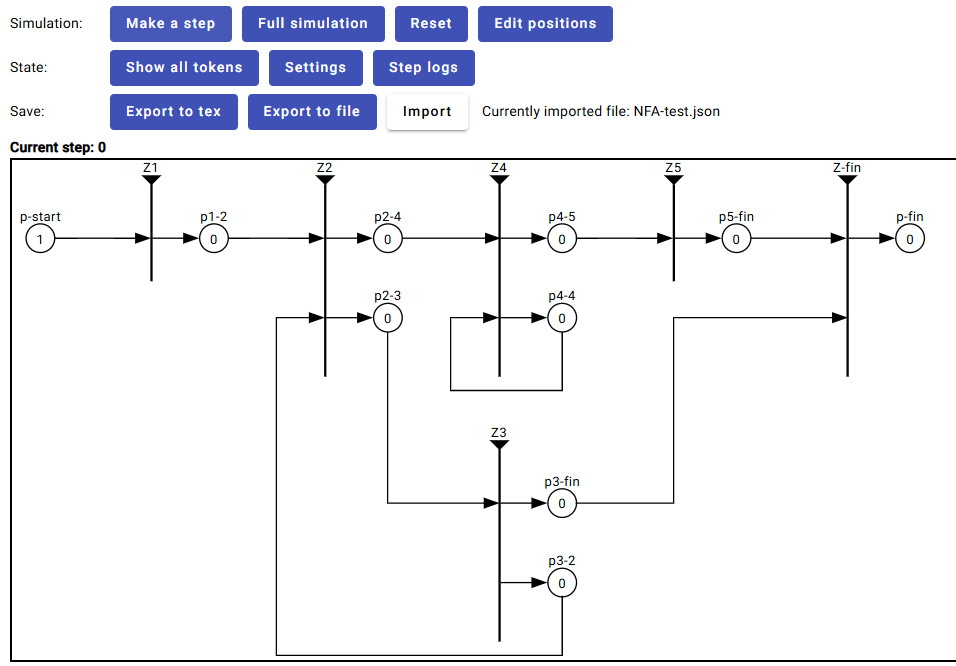
\includegraphics[width=0.9\textwidth]{../../4. applications/finateStateAutomationsGenNets/images/NFA-OGN-1.PNG}}
	\caption*{\textbf{Figure~\ref{DIS-fig:gn_initial_setup}} -- Initial configuration of the generalized net with the starting place ($p_{\text{start}}$).}
\end{figure}

\begin{figure}[H]
	\centering
	\setlength{\fboxrule}{2pt}
	\setlength{\fboxsep}{0pt}
	\fbox{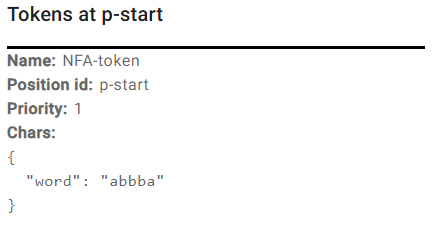
\includegraphics[width=0.55\textwidth]{../../4. applications/finateStateAutomationsGenNets/images/NFA-OGN-2.PNG}}
	\caption*{\textbf{Figure~\ref{DIS-fig:gn_token_start}} -- Token in $p_{\text{start}}$ with characteristic $abbba$.}
\end{figure}

\begin{figure}[H]
	\centering
	\setlength{\fboxrule}{2pt}
	\setlength{\fboxsep}{0pt}
	\fbox{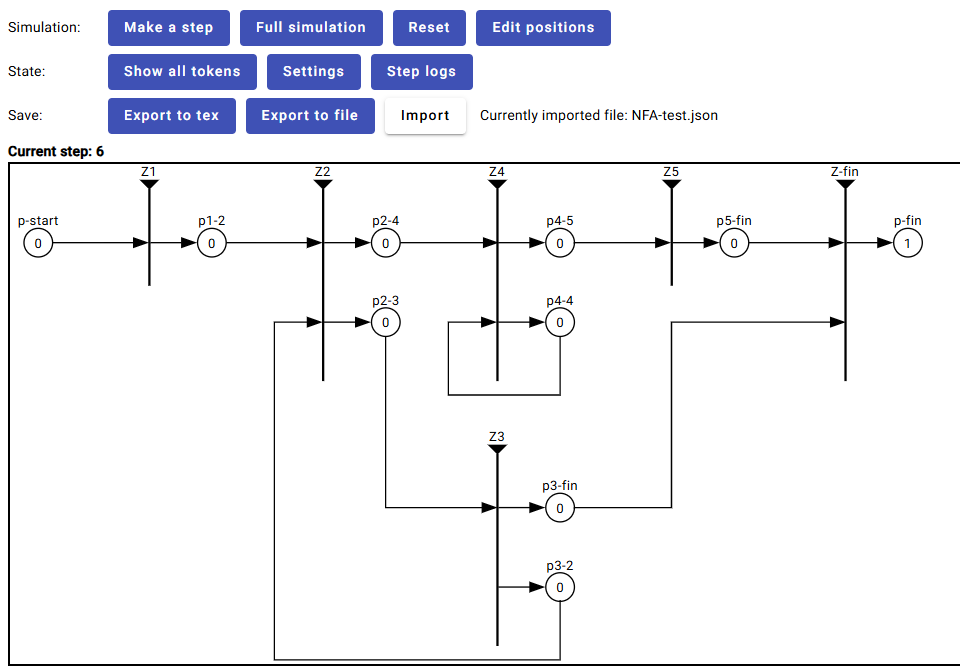
\includegraphics[width=0.9\textwidth]{../../4. applications/finateStateAutomationsGenNets/images/NFA-OGN-5.PNG}}
	\caption*{\textbf{Figure~\ref{DIS-fig:gn_final_state}} -- The token has reached the final place $p_{\text{fin}}$.}
\end{figure}

\begin{figure}[H]
	\centering
	\setlength{\fboxrule}{2pt}
	\setlength{\fboxsep}{0pt}
	\fbox{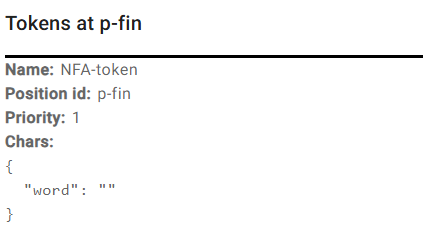
\includegraphics[width=0.55\textwidth]{../../4. applications/finateStateAutomationsGenNets/images/NFA-OGN-6.PNG}}
	\caption*{\textbf{Figure~\ref{DIS-fig:gn_empty_characteristic}} -- The token's characteristic becomes the empty string upon acceptance.}
\end{figure}
	
	\subsubsection{Conclusion}
	
	\hspace*{2.5em}The dissertation considers how GNs can be used for simulation of DFAs and NFAs by associating states with transitions and arcs with places, thus capturing the parallel computation paths. The architecture based on tokens and characteristics allows traceable simulation, while \textit{OnlineGN} is used to demonstrate the execution step by step and to show acceptance clearly (final place and empty characteristic).
	
	
	\subsection{Parallelization of the Towers of Hanoi Problem through Generalized Nets}
	\medskip
	\hspace*{2.5em}A \emph{parallel} version of the classical Towers of Hanoi problem is considered, in which, in one step, simultaneous movement of more than one ring is allowed. The problem is formalized by means of the GN apparatus, and the simulation realization in \textit{OnlineGN} demonstrates the executability of the model and the effect of parallelism in exponential combinatorial processes.
	
	\subsubsection{Description of the Towers of Hanoi Problem}
	\hspace*{2.5em}The classical Towers of Hanoi problem \cite{DIS-wikipediaHanoi} consists of three rods and \(n\) rings of different sizes, initially arranged on the first rod; a larger ring may not be placed on a smaller one (\textbf{Figure~\ref{DIS-fig:fig1}}). The goal is to transfer all rings from the first to the third rod while respecting the rule. When exactly one ring is moved per step, a minimum of \(2^{n}-1\) steps is required \cite{DIS-frame1945,CLRS_TowerOfHanoi}. The present chapter describes the process through GNs.
	
	\subsubsection{{Parallelization of the Towers of Hanoi: Conceptual Overview}\label{sec:parallel-concept}}
	\hspace*{2.5em}The classical constraints are: \textbf{(i)} at each step only one ring is moved and \textbf{(ii)} a larger ring may not be placed on a smaller one. In the parallel variant, \textbf{(i)} is relaxed: in one \emph{parallel step}, a packet of up to \(k\) rings can be \emph{lifted} simultaneously (from the tops of an arbitrary combination of rods), after which they are \emph{placed} one by one according to the priority rule (first the largest, last the smallest). The lift--place cycle counts as one parallel step.
	
	\subsubsection{Configuration of the System}
	\begin{itemize}
		\item \textbf{Rods.}\\
		Three rods \(R_1\) (source), \(R_2\) (auxiliary), \(R_3\) (target), each with a stack of rings in strictly decreasing order of size from bottom to top.
		\item \textbf{Rings.}\\
		\(n\) rings, labeled from \(1\) (smallest) to \(n\) (largest).
		\item \textbf{Air buffer.}\\
		After lifting, the selected up to \(k\) rings are ``in the air'', while the internal order of the rings coming from the same rod is preserved.
	\end{itemize}
	
	\subsubsection{Definition of a Parallel Step}\label{subsec:parallel-step}
	\hspace*{2.5em}Each step has two phases:
	\vspace{-0.1cm}
	\begin{enumerate}
		\item \textbf{Lift phase.} Up to \(k\) rings are selected from the tops of the rods and removed \emph{simultaneously}.
		\item \textbf{Placement phase.} Placement according to the \emph{priority rule}: (1) release in strictly decreasing order of size; (2) placement on an arbitrary rod without violating the local order by size.
	\end{enumerate}
	\hspace*{2.5em}The minimum number of parallel steps is denoted by \(H(n,k)\).
	
	\begin{Theorem}\label{thm:main}
		$H(n,k) = 2^{\bigl\lceil \textstyle \frac{n}{k} \bigr\rceil} - 1$.
	\end{Theorem}
	
	The proof groups the \(n\) rings into \(M=\lceil n/k\rceil\) blocks of size at most \(k\), which are treated as ``super-rings'', and reduces the parallel model to the classical recursion on \(M\) elements (the upper and lower bounds coincide).
	
	\paragraph{Observation (Optimality of block movements in the parallel variant of the Towers of Hanoi).}
	\mbox{}\\
	An optimal strategy always transfers exactly \(k\) consecutive rings from one rod to another; each block behaves as a ``super-ring'', whereby the problem is reduced to the classical Towers of Hanoi on \(\lceil n/k\rceil\) super-rings.
	
	\subsubsection{Generalized-Net Model for the Parallel Towers of Hanoi}
	\hspace*{2.5em}A GN model is introduced for simulation of the \(k\)-parallel rule. The GN contains \(n\) \(\rho\)-tokens (``rings'') and \(k\) \(\chi\)-tokens (``hands''). The \(\chi\)-tokens allow, in one parallel step, at most \(k\) \(\rho\)-tokens to be lifted simultaneously and placed according to the priority rule. The net is constructed so as to realize the optimal block strategy and to be executable in \textit{OnlineGN}.
	
	\begin{figure}[H]
		\tiny  \vspace{30mm}
		%%% Change unitlength and font size to scale the graphic
		%%% Font sizes: \tiny \scriptsize \footnotesize \small \normalsize \large \Large \LARGE \huge \Huge
		\newcommand{\mytriangle}{\Large $\bigtriangledown$}
		\begin{center}
			\setlength{\unitlength}{8.0pt} %10pt=4mm
			\linethickness{0.5pt}
			\begin{picture}(27, 64)
				%%% Transitions
				\put(18.5,71.5){\makebox(0,0)[cc]{$Z_{2}$}}
				\put(20.0,70.0){\makebox(0,0)[bb]{\mytriangle}}
				\put(20.0,70.0){\line(0,-1){25}}
				\put(4.5,51.5){\makebox(0,0)[cc]{$Z_{1}$}}
				\put(6.0,50.0){\makebox(0,0)[bb]{\mytriangle}}
				\put(6.0,50.0){\line(0,-1){25}}
				\put(18.5,31.5){\makebox(0,0)[cc]{$Z_{3}$}}
				\put(20.0,30.0){\makebox(0,0)[bb]{\mytriangle}}
				\put(20.0,30.0){\line(0,-1){25}}
				%%% Input places
				%%% Output places
				\put(21.5,69.5){\makebox(0,0)[cc]{$l_{2,1}$}}
				\put(20.0,68.5){\vector(1,0){1.0}}
				\put(21.5,68.5){\circle{1.0}}
				\put(18.5,67.2){\makebox(0,0)[cc]{$\vdots$}}
				\put(18.5,61.2){\makebox(0,0)[cc]{$\vdots$}}
				\put(18.5,55.2){\makebox(0,0)[cc]{$\vdots$}}
				\put(18.5,49.2){\makebox(0,0)[cc]{$\vdots$}}
				\put(21.5,67.2){\makebox(0,0)[cc]{$\vdots$}}
				\put(21.5,61.2){\makebox(0,0)[cc]{$\vdots$}}
				\put(21.5,55.2){\makebox(0,0)[cc]{$\vdots$}}
				\put(21.5,49.2){\makebox(0,0)[cc]{$\vdots$}}
				\put(21.5,65.5){\makebox(0,0)[cc]{$l_{2,n}$}}
				\put(20.0,64.5){\vector(1,0){1.0}}
				\put(21.5,64.5){\circle{1.0}}
				\put(21.5,63.5){\makebox(0,0)[cc]{$m_{2,1}$}}
				\put(20.0,62.5){\vector(1,0){1.0}}
				\put(21.5,62.5){\circle{1.0}}
				\put(21.5,59.5){\makebox(0,0)[cc]{$m_{2,k}$}}
				\put(20.0,58.5){\vector(1,0){1.0}}
				\put(21.5,58.5){\circle{1.0}}
				\put(21.5,57.5){\makebox(0,0)[cc]{$m_{2,k+1}$}}
				\put(20.0,56.5){\vector(1,0){1.0}}
				\put(21.5,56.5){\circle{1.0}}
				\put(21.5,53.5){\makebox(0,0)[cc]{$m_{2,2k}$}}
				\put(20.0,52.5){\vector(1,0){1.0}}
				\put(21.5,52.5){\circle{1.0}}
				\put(21.8,51.5){\makebox(0,0)[cc]{$m_{2,k+1}$}}
				\put(20.0,50.5){\vector(1,0){1.0}}
				\put(21.5,50.5){\circle{1.0}}
				\put(7.5,49.5){\makebox(0,0)[cc]{$l_{1,1}$}}
				\put(6.0,48.5){\vector(1,0){1.0}}
				\put(7.5,48.5){\circle{1.0}}
				\put(7.5,47.2){\makebox(0,0)[cc]{$\vdots$}}
				\put(4.5,47.2){\makebox(0,0)[cc]{$\vdots$}}
				\put(7.5,41.2){\makebox(0,0)[cc]{$\vdots$}}
				\put(4.5,41.2){\makebox(0,0)[cc]{$\vdots$}}
				\put(7.5,35.2){\makebox(0,0)[cc]{$\vdots$}}
				\put(4.5,35.2){\makebox(0,0)[cc]{$\vdots$}}
				\put(7.5,29.2){\makebox(0,0)[cc]{$\vdots$}}
				\put(4.5,29.2){\makebox(0,0)[cc]{$\vdots$}}
				\put(21.5,47.5){\makebox(0,0)[cc]{$m_{2,2k}$}}
				\put(20.0,46.5){\vector(1,0){1.0}}
				\put(21.5,46.5){\circle{1.0}}
				\put(7.5,45.5){\makebox(0,0)[cc]{$l_{1,n}$}}
				\put(6.0,44.5){\vector(1,0){1.0}}
				\put(7.5,44.5){\circle{1.0}}
				\put(7.5,43.5){\makebox(0,0)[cc]{$m_{1,k+1}$}}
				\put(6.0,42.5){\vector(1,0){1.0}}
				\put(7.5,42.5){\circle{1.0}}
				\put(7.5,39.5){\makebox(0,0)[cc]{$m_{1,2k}$}}
				\put(6.0,38.5){\vector(1,0){1.0}}
				\put(7.5,38.5){\circle{1.0}}
				\put(7.5,37.5){\makebox(0,0)[cc]{$m_{1,2k+1}$}}
				\put(6.0,36.5){\vector(1,0){1.0}}
				\put(7.5,36.5){\circle{1.0}}
				\put(7.5,33.5){\makebox(0,0)[cc]{$m_{1,3k}$}}
				\put(6.0,32.5){\vector(1,0){1.0}}
				\put(7.5,32.5){\circle{1.0}}
				\put(7.8,31.5){\makebox(0,0)[cc]{$m_{1,1}$}}
				\put(6.0,30.5){\vector(1,0){1.0}}
				\put(7.5,30.5){\circle{1.0}}
				\put(21.5,29.5){\makebox(0,0)[cc]{$l_{3,1}$}}
				\put(20.0,28.5){\vector(1,0){1.0}}
				\put(21.5,28.5){\circle{1.0}}
				\put(21.5,27.2){\makebox(0,0)[cc]{$\vdots$}}
				\put(18.5,27.2){\makebox(0,0)[cc]{$\vdots$}}
				\put(21.5,21.2){\makebox(0,0)[cc]{$\vdots$}}
				\put(18.5,21.2){\makebox(0,0)[cc]{$\vdots$}}
				\put(21.5,15.2){\makebox(0,0)[cc]{$\vdots$}}
				\put(18.5,15.2){\makebox(0,0)[cc]{$\vdots$}}
				\put(21.5,9.2){\makebox(0,0)[cc]{$\vdots$}}
				\put(18.5,9.2){\makebox(0,0)[cc]{$\vdots$}}
				\put(7.5,27.5){\makebox(0,0)[cc]{$m_{1,k}$}}
				\put(6.0,26.5){\vector(1,0){1.0}}
				\put(7.5,26.5){\circle{1.0}}
				\put(21.5,25.5){\makebox(0,0)[cc]{$l_{3,n}$}}
				\put(20.0,24.5){\vector(1,0){1.0}}
				\put(21.5,24.5){\circle{1.0}}
				\put(21.5,23.5){\makebox(0,0)[cc]{$m_{3,k+1}$}}
				\put(20.0,22.5){\vector(1,0){1.0}}
				\put(21.5,22.5){\circle{1.0}}
				\put(21.5,19.5){\makebox(0,0)[cc]{$m_{3,2k}$}}
				\put(20.0,18.5){\vector(1,0){1.0}}
				\put(21.5,18.5){\circle{1.0}}
				\put(21.8,17.5){\makebox(0,0)[cc]{$m_{3,1}$}}
				\put(20.0,16.5){\vector(1,0){1.0}}
				\put(21.5,16.5){\circle{1.0}}
				\put(21.5,13.5){\makebox(0,0)[cc]{$m_{3,k}$}}
				\put(20.0,12.5){\vector(1,0){1.0}}
				\put(21.5,12.5){\circle{1.0}}
				\put(21.8,11.5){\makebox(0,0)[cc]{$m_{3,2k+1}$}}
				\put(20.0,10.5){\vector(1,0){1.0}}
				\put(21.5,10.5){\circle{1.0}}
				\put(21.5,7.5){\makebox(0,0)[cc]{$m_{3,3k}$}}
				\put(20.0,6.5){\vector(1,0){1.0}}
				\put(21.5,6.5){\circle{1.0}}
				%%% Vertical paths
				\put(0.5,75.5){\line(0,-1){37}}
				\put(25.5,75.5){\line(0,-1){17}}
				\put(1.5,74.5){\line(0,-1){32}}
				\put(24.5,74.5){\line(0,-1){12}}
				\put(16.5,73.5){\line(0,-1){9}}
				\put(23.5,73.5){\line(0,-1){9}}
				\put(17.5,72.5){\line(0,-1){4}}
				\put(22.5,72.5){\line(0,-1){4}}
				\put(10.5,62.5){\line(0,-1){20}}
				\put(13.5,58.5){\line(0,-1){20}}
				\put(14.5,56.5){\line(0,-1){20}}
				\put(26.5,56.5){\line(0,-1){22}}
				\put(2.5,53.5){\line(0,-1){9}}
				\put(9.5,53.5){\line(0,-1){9}}
				\put(3.5,52.5){\line(0,-1){4}}
				\put(8.5,52.5){\line(0,-1){4}}
				\put(15.5,52.5){\line(0,-1){11}}
				\put(25.5,52.5){\line(0,-1){15}}
				\put(16.5,50.5){\line(0,-1){8}}
				\put(23.5,50.5){\line(0,-1){8}}
				\put(17.5,46.5){\line(0,-1){3}}
				\put(22.5,46.5){\line(0,-1){3}}
				\put(24.5,41.5){\line(0,-1){23}}
				\put(15.5,37.5){\line(0,-1){19}}
				\put(0.5,36.5){\line(0,-1){36}}
				\put(11.5,36.5){\line(0,-1){20}}
				\put(25.5,36.5){\line(0,-1){14}}
				\put(14.5,34.5){\line(0,-1){12}}
				\put(16.5,33.5){\line(0,-1){9}}
				\put(23.5,33.5){\line(0,-1){9}}
				\put(1.5,32.5){\line(0,-1){31}}
				\put(10.5,32.5){\line(0,-1){20}}
				\put(17.5,32.5){\line(0,-1){4}}
				\put(22.5,32.5){\line(0,-1){4}}
				\put(2.5,30.5){\line(0,-1){8}}
				\put(9.5,30.5){\line(0,-1){8}}
				\put(3.5,26.5){\line(0,-1){3}}
				\put(8.5,26.5){\line(0,-1){3}}
				\put(25.5,16.5){\line(0,-1){16}}
				\put(24.5,12.5){\line(0,-1){11}}
				\put(16.5,10.5){\line(0,-1){8}}
				\put(23.5,10.5){\line(0,-1){8}}
				\put(17.5,6.5){\line(0,-1){3}}
				\put(22.5,6.5){\line(0,-1){3}}
				%%% Horizontal paths
				\put(0.5,75.5){\line(1,0){25}}
				\put(1.5,74.5){\line(1,0){23}}
				\put(16.5,73.5){\line(1,0){7}}
				\put(17.5,72.5){\line(1,0){5}}
				\put(17.5,68.5){\vector(1,0){2.5}}
				\put(16.5,64.5){\vector(1,0){3.5}}
				\put(10.5,62.5){\vector(1,0){9.5}}
				\put(13.5,58.5){\vector(1,0){6.5}}
				\put(14.5,56.5){\vector(1,0){5.5}}
				\put(2.5,53.5){\line(1,0){7}}
				\put(3.5,52.5){\line(1,0){5}}
				\put(15.5,52.5){\vector(1,0){4.5}}
				\put(16.5,50.5){\vector(1,0){3.5}}
				\put(3.5,48.5){\vector(1,0){2.5}}
				\put(17.5,46.5){\vector(1,0){2.5}}
				\put(2.5,44.5){\vector(1,0){3.5}}
				\put(17.5,43.5){\line(1,0){5}}
				\put(1.5,42.5){\vector(1,0){4.5}}
				\put(16.5,42.5){\line(1,0){7}}
				\put(15.5,41.5){\line(1,0){9}}
				\put(0.5,38.5){\vector(1,0){5.5}}
				\put(15.5,37.5){\line(1,0){10}}
				\put(0.5,36.5){\vector(1,0){5.5}}
				\put(14.5,36.5){\line(1,0){11}}
				\put(14.5,34.5){\line(1,0){12}}
				\put(16.5,33.5){\line(1,0){7}}
				\put(1.5,32.5){\vector(1,0){4.5}}
				\put(17.5,32.5){\line(1,0){5}}
				\put(2.5,30.5){\vector(1,0){3.5}}
				\put(17.5,28.5){\vector(1,0){2.5}}
				\put(3.5,26.5){\vector(1,0){2.5}}
				\put(16.5,24.5){\vector(1,0){3.5}}
				\put(3.5,23.5){\line(1,0){5}}
				\put(2.5,22.5){\line(1,0){7}}
				\put(14.5,22.5){\vector(1,0){5.5}}
				\put(15.5,18.5){\vector(1,0){4.5}}
				\put(11.5,16.5){\vector(1,0){8.5}}
				\put(10.5,12.5){\vector(1,0){9.5}}
				\put(16.5,10.5){\vector(1,0){3.5}}
				\put(17.5,6.5){\vector(1,0){2.5}}
				\put(17.5,3.5){\line(1,0){5}}
				\put(16.5,2.5){\line(1,0){7}}
				\put(1.5,1.5){\line(1,0){23}}
				\put(0.5,0.5){\line(1,0){25}}
				%%% Horizontal paths from output places
				\put(22.0,64.5){\line(1,0){1.5}}
				\put(22.0,62.5){\line(1,0){2.5}}
				\put(22.0,58.5){\line(1,0){3.5}}
				\put(22.0,56.5){\line(1,0){4.5}}
				\put(22.0,52.5){\line(1,0){3.5}}
				\put(22.0,50.5){\line(1,0){1.5}}
				\put(8.0,44.5){\line(1,0){1.5}}
				\put(8.0,42.5){\line(1,0){2.5}}
				\put(8.0,38.5){\line(1,0){5.5}}
				\put(8.0,36.5){\line(1,0){3.5}}
				\put(8.0,32.5){\line(1,0){2.5}}
				\put(8.0,30.5){\line(1,0){1.5}}
				\put(22.0,24.5){\line(1,0){1.5}}
				\put(22.0,22.5){\line(1,0){3.5}}
				\put(22.0,18.5){\line(1,0){2.5}}
				\put(22.0,16.5){\line(1,0){3.5}}
				\put(22.0,12.5){\line(1,0){2.5}}
				\put(22.0,10.5){\line(1,0){1.5}}
				%%% Corners
				\put(22.0,68.5){\line(1,0){0.5}}
				\put(8.0,48.5){\line(1,0){0.5}}
				\put(22.0,46.5){\line(1,0){0.5}}
				\put(22.0,28.5){\line(1,0){0.5}}
				\put(8.0,26.5){\line(1,0){0.5}}
				\put(22.0,6.5){\line(1,0){0.5}}
			\end{picture}
		\end{center}
		\normalsize
		\caption*{\textbf{Figure~\ref{DIS-fig:gn_th_rho_chi_tokens}} -- Generalized Net for the Tower of Hanoi: $n \rho$-tokens and $k \chi$-tokens.}
	\end{figure} % Figure 12
	
	\subsubsection*{Tokens and movements.}
	\vspace{-0.1cm}
	\hspace*{2.5em}The following conventions are used:
	\vspace{-0.2cm}
	\begin{itemize}
		\item \(\rho\)-token: ring; initial characteristic -- the size.
		\item \(\chi\)-token: ``hand''; characteristic -- the index of the ``hand''.
	\end{itemize}
	\hspace*{2.5em}A distinction is made between a \emph{move of the puzzle} and a \emph{net move}. Each move of the puzzle is realized by \textbf{two net moves}: (i) positioning the \(\rho\)- and \(\chi\)-tokens at the output places of the transition of the source rod; (ii) transferring them to the input--output places of the transition of the target rod. In this way, the GN simulates the transfer of \(\rho\)-tokens between rods through a sequence of net moves.
	
	\subsubsection*{Transitions and places.}
	\vspace{-0.1cm}
	\hspace*{2.5em}The GN contains \textbf{three transitions} \(Z_1\), \(Z_2\), \(Z_3\) (one for each rod). For the \(\rho\)-tokens, \(n\) \textbf{input--output places} \(l_{i,j}\) (\(i\in\{1,2,3\}\), \(j=1,\dots,n\)) are used; a \(\rho\)-token in \(l_{i,j}\) means ``a ring of size \(j\) is on rod \(i\)''. For the \(\chi\)-tokens, \textbf{holding places} \(m_{i,j}\) (\(j\in[1,3k]\)) are used, which encode the current/next rod for taking and transferring, depending on the parity of the net step. The general form of the GN is shown in \textbf{Figure~\ref{DIS-fig:gn_th_rho_chi_tokens}}.
	
	\subsubsection*{Indexed matrices.}
	\vspace{-0.1cm}
	\hspace*{2.5em}The predicates over the indexed matrices of the GN are:
	\vspace{-0.2cm}
	\begin{itemize}
		\item \(U_{x,y}\): ``a \(\rho\)-token is moved from \(x\) to \(y\) in this step of the puzzle'';
		\item \(W_{x,y,i,j}\): selection of a \(\chi\)-token for moving a \(\rho\)-token and ensuring the correct position in the block mode;
		\item \(P_i\): ``a \(\rho\)-token has characteristic weight \(i\)'' (correct positioning after the move);
		\item \(S_x\): placing the \(\chi\)-tokens in output places according to the forthcoming move.
	\end{itemize}
	\hspace*{2.5em}The indexed matrices for odd and even net moves are given in \textbf{Figures~\ref{DIS-fig:block-matrix} and~\ref{DIS-fig:index-matrix-even-net-moves}}.
	
\begin{figure}[H]
	\centering
	\small
	% narrowing the block
	\begin{adjustwidth}{\extralength}{\extralength}
		% denser columns
		\setlength{\arraycolsep}{3pt}%
		\renewcommand{\arraystretch}{1.05}%
		\[
		% ensure it doesn't exceed the linewidth
		\resizebox{1\linewidth}{!}{$
			\begin{array}{c|cccccccccccc}
				& l_{a,1} & \cdots & l_{a,n} & m_{a,(a-1)*k + 1} & \cdots & m_{a,a * k} & m_{a,(b-1)*k + 1} & \cdots & m_{a,b*k} & m_{a,(c-1)*k + 1} & \cdots & m_{a,c*k} \\ \hline
				l_{a,1} & F & \cdots & F & F & \cdots & F & W_{a,b,1, 1} & \cdots & W_{a,b,1, k} & W_{a,c,1, 1} & \cdots & W_{a,c,n, k} \\
				\vdots &  \vdots & \ddots &  \vdots &  \vdots & \ddots &  \vdots &  \vdots & \ddots &  \vdots &  \vdots & \ddots &  \vdots \\
				l_{a,n} & F & \cdots & F & F & \cdots & F & W_{a,b,n, 1} & \cdots & W_{a,b,n, k} & W_{a,c,n, 1} & \cdots & W_{a,c,n, k} \\
				m_{a,(a-1)*k + 1} & F & \cdots & F & F & \cdots & F & U_{a,b} & \cdots & F & U_{a,c} & \cdots & F \\
				\vdots & \vdots & \ddots & \vdots & \vdots & \ddots & \vdots & \vdots & \ddots & \vdots & \vdots & \ddots & \vdots \\
				m_{a,a*k} & F & \cdots & F & F & \cdots & F & F & \cdots & U_{a,b} & F & \cdots & U_{a,c} \\
				m_{b,(a-1)*k + 1} & F & \cdots & F & F & \cdots & F & U_{a,b} & \cdots & F & U_{a,c} & \cdots & F \\
				\vdots & \vdots & \ddots & \vdots & \vdots & \ddots & \vdots & \vdots & \ddots & \vdots & \vdots & \ddots & \vdots \\
				m_{b,a*k} & F & \cdots & F & F & \cdots & F & F & \cdots & U_{a,b} & F & \cdots & U_{a,c} \\
				m_{c,(a-1)*k + 1} & F & \cdots & F & F & \cdots & F & U_{a,b} & \cdots & F & U_{a,c} & \cdots & F \\
				\vdots & \vdots & \ddots & \vdots & \vdots & \ddots & \vdots & \vdots & \ddots & \vdots & \vdots & \ddots & \vdots \\
				m_{c,a*k} & F & \cdots & F & F & \cdots & F & F & \cdots & U_{a,b} & F & \cdots & U_{a,c}
			\end{array}
			$}
		\]
	\end{adjustwidth}
	\caption*{\textbf{Figure~\ref{DIS-fig:block-matrix}} -- Indexed matrix of $Z_X$ for the odd network moves (beginning of a puzzle move).}
\end{figure}


\begin{figure}[H]
	\centering
	\small
	% narrowing the block symmetrically
	\begin{adjustwidth}{\extralength}{\extralength}
		\setlength{\arraycolsep}{3pt}%
		\renewcommand{\arraystretch}{1.05}%
		\[
		\resizebox{1\linewidth}{!}{$
			\begin{array}{c|cccccccccccc}
				& l_{a,1} & \cdots & l_{a,n} & m_{a,(a-1)*k + 1} & \cdots & m_{a,a * k} & m_{a,(b-1)*k + 1} & \cdots & m_{a,b*k} & m_{a,(c-1)*k + 1} & \cdots & m_{a,c*k} \\ \hline
				l_{a,1} & F & \cdots & F & F & \cdots & F & F & \cdots & F & F & \cdots & F \\
				\vdots  & \vdots & \ddots & \vdots & \vdots & \ddots & \vdots & \vdots & \ddots & \vdots & \vdots & \ddots & \vdots \\
				l_{a,n} & F & \cdots & F & F & \cdots & F & F & \cdots & F & F & \cdots & F \\
				m_{a,(a-1)*k + 1} & F & \cdots & F & F & \cdots & F & F & \cdots & F & F & \cdots & F \\
				\vdots  & \vdots & \ddots & \vdots & \vdots & \ddots & \vdots & \vdots & \ddots & \vdots & \vdots & \ddots & \vdots \\
				m_{a,a*k} & F & \cdots & F & F & \cdots & F & F & \cdots & F & F & \cdots & F \\
				m_{b,(a-1)*k + 1} & P_{1} & \cdots & P_{n} & S_{a} & \cdots & F & S_{b} & \cdots & F & S_{c} & \cdots & F \\
				\vdots  & \vdots & \ddots & \vdots & \vdots & \ddots & \vdots & \vdots & \ddots & \vdots & \vdots & \ddots & \vdots \\
				m_{b,a*k} & P_{1} & \cdots & P_{n} & F & \cdots & S_{a} & F & \cdots & S_{b} & F & \cdots & S_{c} \\
				m_{c,(a-1)*k + 1} & P_{1} & \cdots & P_{n} & S_{a} & \cdots & F & S_{b} & \cdots & F & S_{c} & \cdots & F \\
				\vdots  & \vdots & \ddots & \vdots & \vdots & \ddots & \vdots & \vdots & \ddots & \vdots & \vdots & \ddots & \vdots \\
				m_{c,a*k} & P_{1} & \cdots & P_{n} & F & \cdots & S_{a} & F & \cdots & S_{b} & F & \cdots & S_{c}
			\end{array}
			$}
		\]
	\end{adjustwidth}
	\caption*{\textbf{Figure~\ref{DIS-fig:index-matrix-even-net-moves}} -- Indexed matrix of $Z_X$ for the even network moves (end of a puzzle move).}
\end{figure}
	
	\begin{Theorem}
		The GN describing the Hanoi puzzle with \(n\) \(\rho\)-tokens and \(k\) \(\chi\)-tokens transfers the \(\rho\)-tokens from the first to the third rod in \(2^{\bigl\lceil \textstyle \frac{n}{k} \bigr\rceil} - 1\) moves of the puzzle.
	\end{Theorem}
	
	The proof is a direct application of \textbf{Theorem~\ref{thm:main}} for \(N=n\), \(K=k\), through grouping the \(\rho\)-tokens into blocks of size at most \(k\).
	
	\subsubsection{Simulations with \textit{OnlineGN}}
	\hspace*{2.5em}The developed GN model has been simulated with \textit{OnlineGN}. Due to the size of the net, screenshots are used that show the active segments. For the example \(n=3\), \(k=2\), the initial configuration has the \(\rho\)- and \(\chi\)-tokens at \(Z_1\) (\textbf{Figure~\ref{DIS-fig:step1}}), after which intermediate positioning toward \(m\)-places directed to \(Z_2\) is observed (\textbf{Figure~\ref{DIS-fig:step2}}), and a final configuration with all \(\rho\)-tokens in \(Z_3\) (\textbf{Figure~\ref{DIS-fig:final_step}}). For all tested pairs \((n,k)\), the reported number of steps coincides with \(2^{\lceil n/k\rceil}-1\).
	
	\vspace{0.3cm}
	
\begin{figure}[H]
	\centering
	\setlength{\fboxrule}{2pt}
	\setlength{\fboxsep}{0pt}
	\fbox{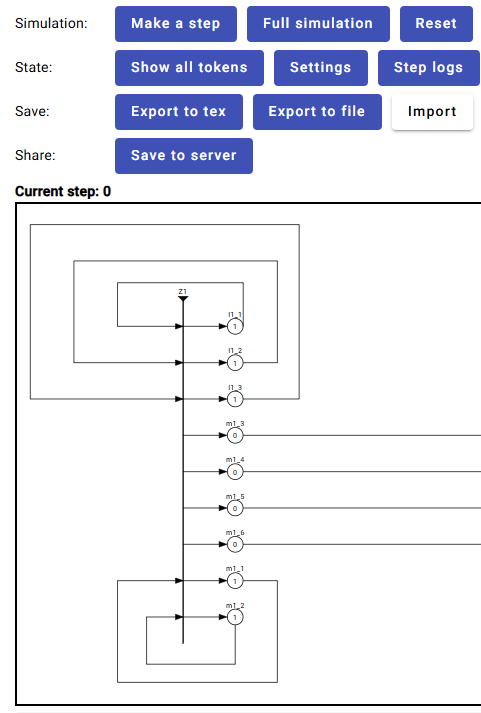
\includegraphics[width=0.6\textwidth]{../../4. applications/hanoiTowers/images/s1_1.png}}
	\captionsetup{width=0.8\textwidth}
	\caption*{\textbf{Figure~\ref{DIS-fig:step1}} -- Generalized Net for the Tower of Hanoi with 3 $\rho$-tokens and 2 $\chi$-tokens in OnlineGN.}
\end{figure}


\begin{figure}[H]
	\centering
	\setlength{\fboxrule}{2pt}
	\setlength{\fboxsep}{0pt}
	\fbox{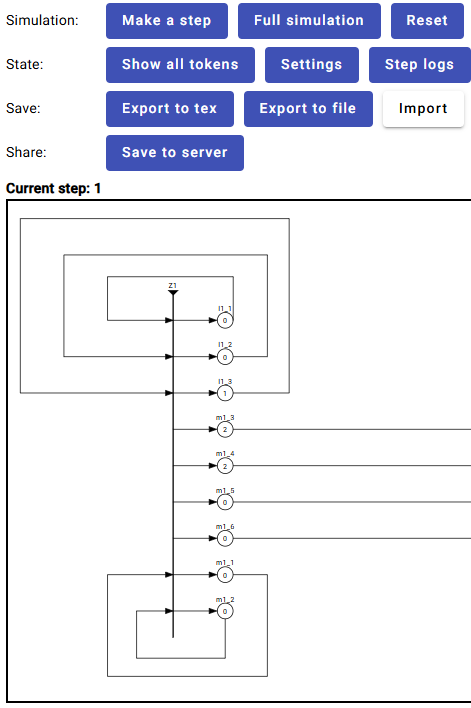
\includegraphics[width=0.6\textwidth]{../../4. applications/hanoiTowers/images/s2_1.png}}
	\captionsetup{width=0.8\textwidth}
	\caption*{\textbf{Figure~\ref{DIS-fig:step2}} -- The $\rho$- and $\chi$-tokens are positioned for movement to the next transition (rod).}
\end{figure}

\begin{figure}[H]
	\centering
	\setlength{\fboxrule}{2pt}
	\setlength{\fboxsep}{0pt}
	\fbox{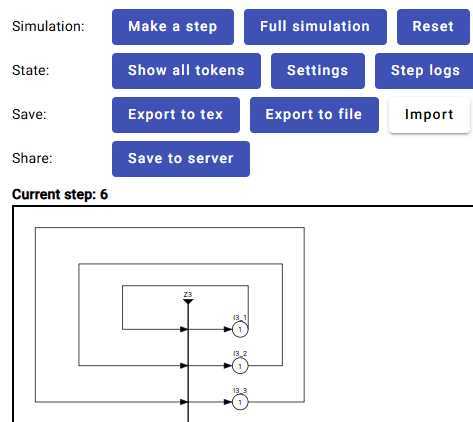
\includegraphics[width=0.6\textwidth]{../../4. applications/hanoiTowers/images/s3_1.png}}
	\captionsetup{width=0.8\textwidth}
	\caption*{\textbf{Figure~\ref{DIS-fig:final_step}} -- Final configuration: all $\rho$-tokens occupy the output positions of $Z_3$ (Tower of Hanoi interpretation: third rod).}
\end{figure}
	
	\subsubsection{Other Studies on Parallel Solving of Problems}
	\hspace*{2.5em}Other parallel solutions of exponential problems are considered.
	
	\subsubsection{Conclusions from the Results}
	\hspace*{2.5em}The developed GN is a direct, executable model of the \(k\)-parallel rule of the Towers of Hanoi. When executed in \textbf{\textit{OnlineGN}}, the simulation generates the expected number of moves \(2^{\bigl\lceil \textstyle \frac{n}{k} \bigr\rceil} - 1\) for all tested \(n\) and \(k\), which confirms the correctness and numerical validity of the model. Increasing \(k\) shortens the critical path, but the gains decrease because of the cost of synchronization (lifting and placing under a global constraint on the order), i.e.\ the process is \emph{synchronization-limited}.
	
	\subsection{Generalized-Net Model of the Production of Gas and Polymeric Products in a Petroleum Refinery}
	
	\hspace*{2.5em}The dissertation considers a GN model of the production of fuel gas, LPG (\textit{LPG}), propylene, and polypropylene, and its software simulation through \textit{OnlineGN}. The construction of the model and the details of the formalization are presented in \cite{DIS-Stratiev2023_1}.
	
	\subsubsection{Introduction to the Production of Products in a Petroleum Refinery}
	
	\hspace*{2.5em}Modeling the processes of production of refined products in a petroleum refinery supports production planning and analysis of efficiency. In the literature, partial models of separate aspects of the problem can be found \cite{DIS-Zhou2017, Infosys2018, 40}, whereas in GNs the cause--effect dependencies are specified through the predicates of the transitions and the characteristics of the tokens.
	
	In previous studies \cite{DIS-87,DIS-88} it has been shown that the production of automotive gasoline \cite{DIS-87} and diesel fuel \cite{DIS-88} can be modeled through GNs; the present chapter complements this line with the production of fuel gas, \textit{LPG}, propylene, and polypropylene and its verification through \textit{OnlineGN}.
	
	\subsubsection{Technological Scheme for the Production of Fuel Gas, LPG, Propylene, and Polypropylene in a Petroleum Refinery}
	
	\hspace*{2.5em}The technological production chain for fuel gas, LPG, propylene, and polypropylene is presented in \textbf{Figure~\ref{DIS-H}} (in the dissertation it is used as a basis for formalization in GNs).
	
\begin{figure}[H]
	\centering
	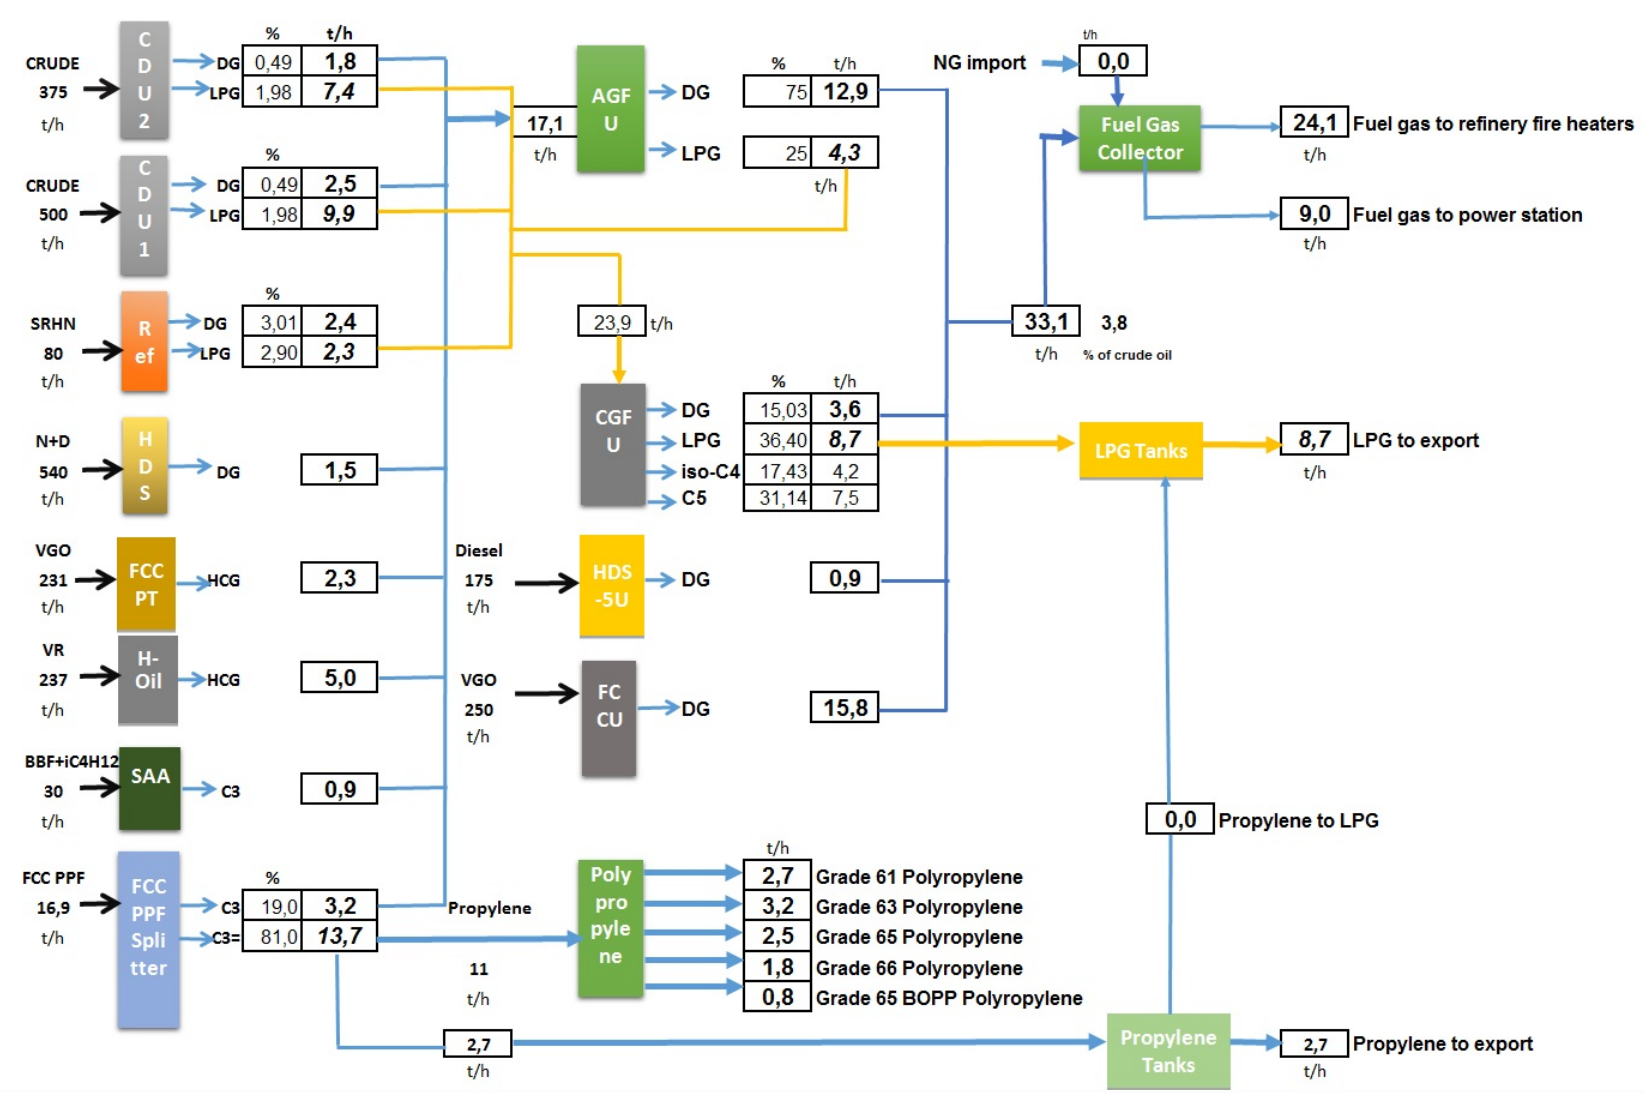
\includegraphics[scale=0.48]{../../4. applications/fuelGasEtc/images/Figure1.png}
	\caption*{\textbf{Figure~\ref{DIS-H}} -- Processing scheme of fuel gas, LPG, propylene, and polypropylene production in a petroleum refinery.}
\end{figure}
	
	The production of petroleum gas products depends on the origin of the crude oil and the operating regimes in the process units. Depending on market requirements, the liquid propylene may be exported as polymer-grade propylene or used as a component of LPG; the polypropylene unit produces various grades of polypropylene products.
	
	\subsubsection{Main Results: Generalized-Net Model}
	
	\hspace*{2.5em}The dissertation considers the GN model (\textbf{Figure~\ref{DIS-fig3}}), which describes the technological chain under consideration through places, transitions, and tokens with characteristics. The model contains 17 transitions, 55 places, and 47 token types, including: streams of raw materials/intermediate fractions ($\sigma_i$), process units ($\rho_i$), and products ($\alpha$, $\beta$, $\gamma$, $\delta$, $\varepsilon$), according to \cite{DIS-Stratiev2023_1}.
	
\begin{figure}[H]
	\centering
	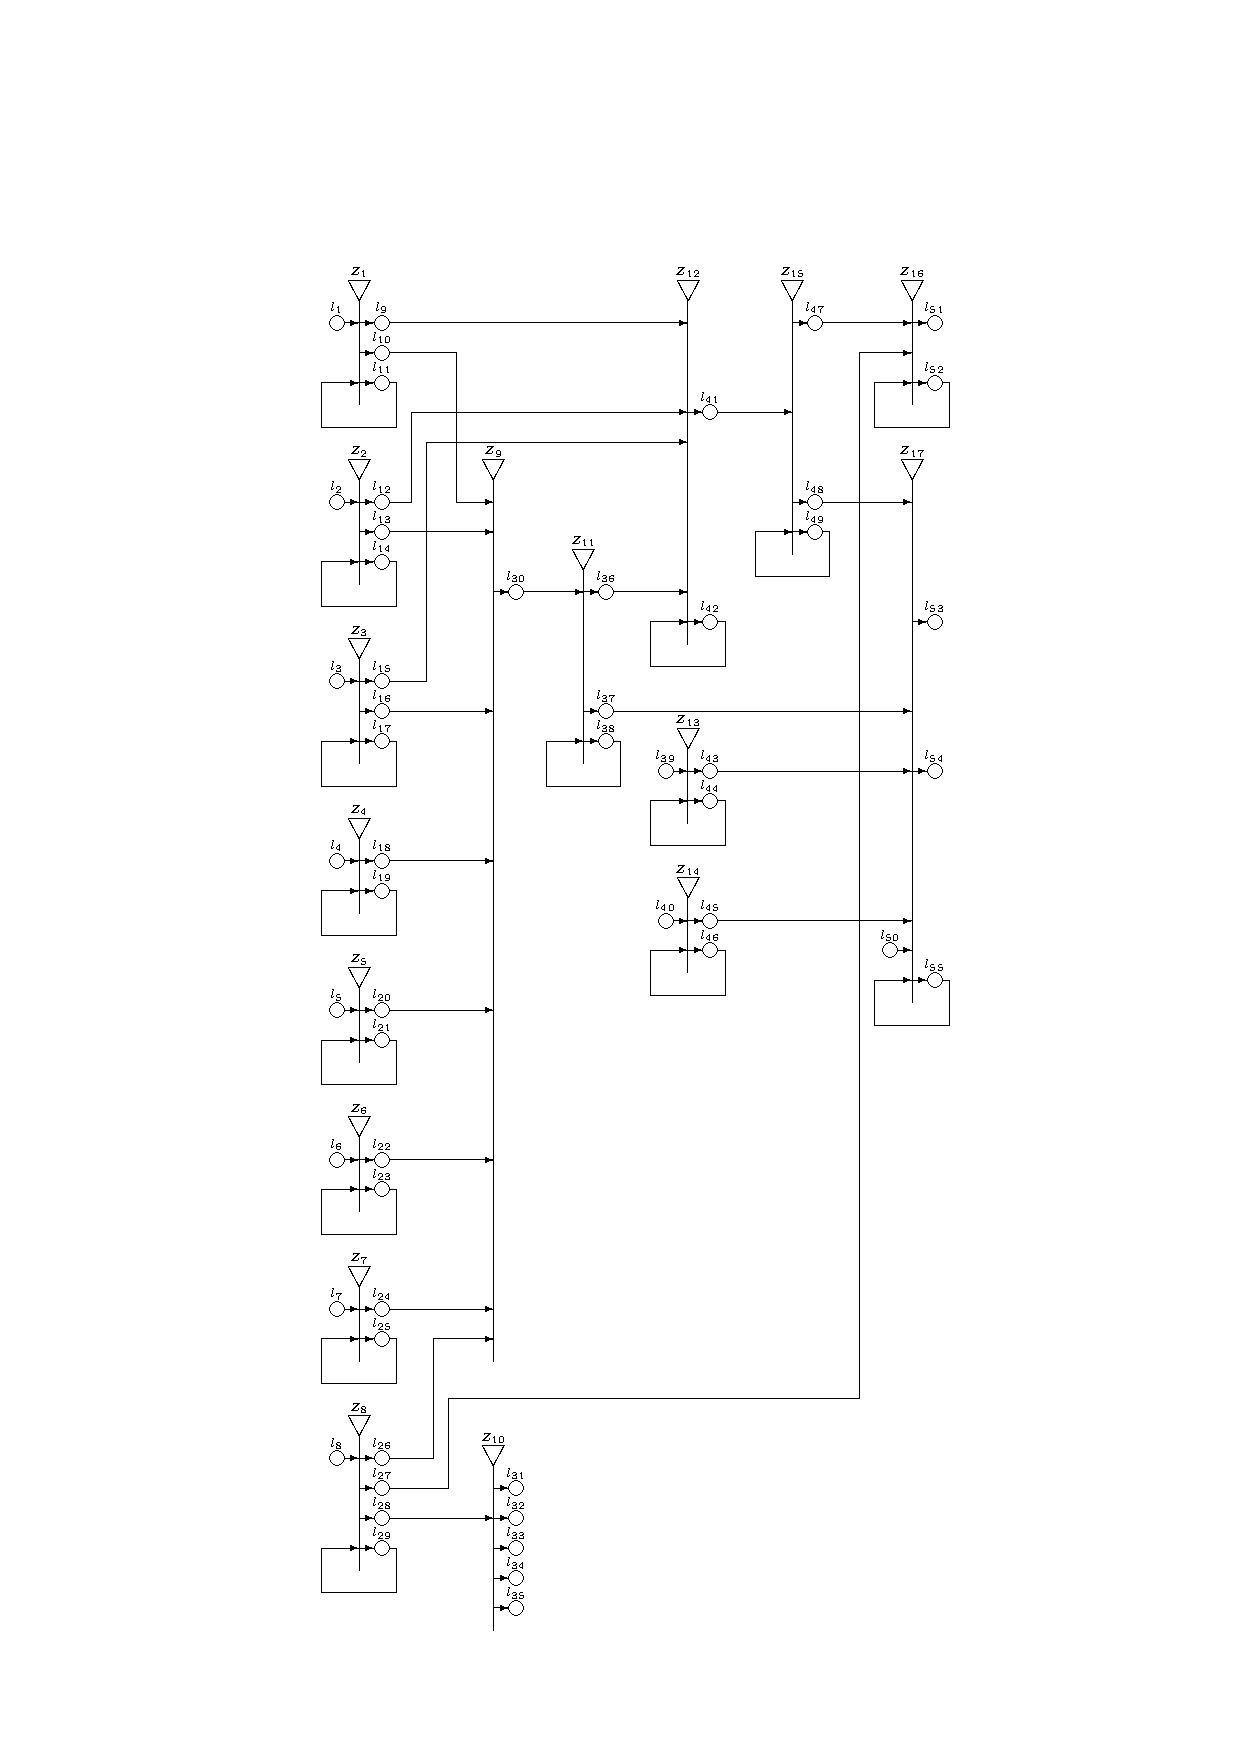
\includegraphics[width=10.1cm]{../../4. applications/fuelGasEtc/images/Figure3.pdf}
	\caption*{\textbf{Figure~\ref{DIS-fig3}} -- Generalized net model.}
\end{figure}
	
	The logic of the process is defined through indexed matrices with predicates for each transition (e.g. conditions of the type ``there is a request for product ...''), which determine the movement of tokens from the input to the output places and the change of their characteristics during simulation.
	
	\subsubsection{Remarks on the Results and the Generalized-Net Model}
	
	\hspace*{2.5em}The production of fuel gas, \textit{LPG}, propylene, and polypropylene is a complex parallel process with multiple technological units and constraints, which can be represented through GNs.
	
	\subsubsection{Simulation with \textit{OnlineGN}}
	\label{subsec:simulation-onlinegn}
	
	\hspace*{2.5em}In order to verify in practice whether the proposed GN model correctly describes the process of production of fuel gas, \textit{LPG}, propylene, and polypropylene in a petroleum refinery, we implemented and simulated it in \textit{OnlineGN}. In this way, we obtain not only a visualization of the structure (places, transitions, and connections), but also the possibility to trace how the tokens ``move'' and how their characteristics change when passing through the separate units.
	
	Due to the size of the model, its visual representation is divided into three parts: upper, middle, and lower. Here, only the upper part is shown in \textbf{Figure~\ref{DIS-fig:onlinegn-model-upper}}.
	
\begin{figure}[H]
	\centering
	\setlength{\fboxrule}{2pt}
	\setlength{\fboxsep}{0pt}
	\fbox{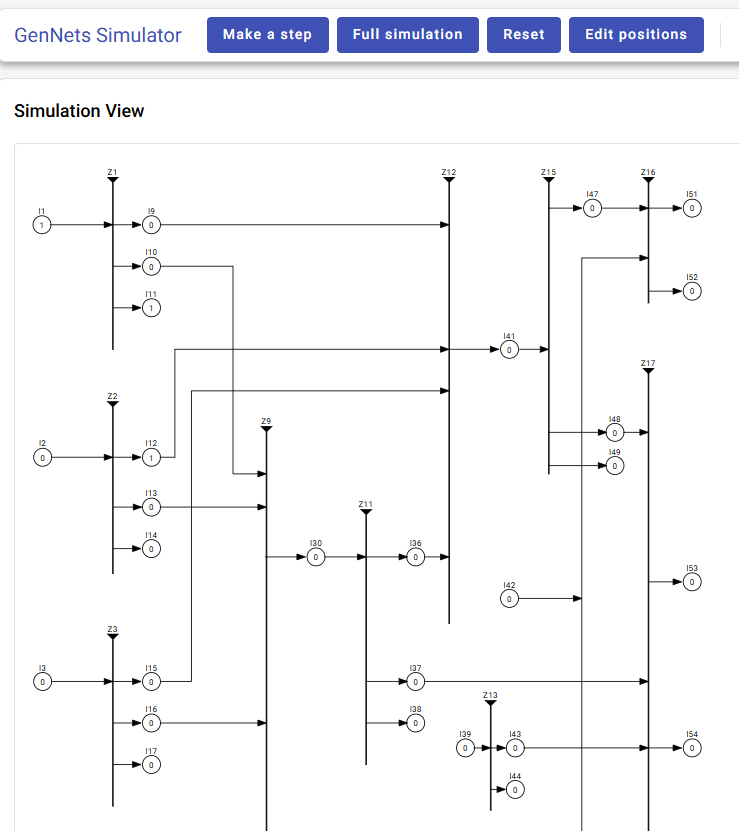
\includegraphics[width=0.95\linewidth]{../../4. applications/fuelGasEtc/images/upper.png}}
	\caption*{\textbf{Figure~\ref{DIS-fig:onlinegn-model-upper}} -- Upper part of the generalized net model in OnlineGN.}
\end{figure}
	
	The next important step is the logic of the transitions: for each transition, indexed matrices are defined in which the predicates from the theoretical description are embedded. It is precisely these predicates that ``decide'' whether a given token can pass from the input to the output places of the transition. In \textbf{Figure~\ref{DIS-fig:onlinegn-matrix-z1}} an example is shown with an indexed matrix for transition $Z_1$, which in the model corresponds to \textit{CDU-2}.
	
	\begin{figure}[H]
		\centering
		\setlength{\fboxrule}{2pt}
		\setlength{\fboxsep}{0pt}
		\fbox{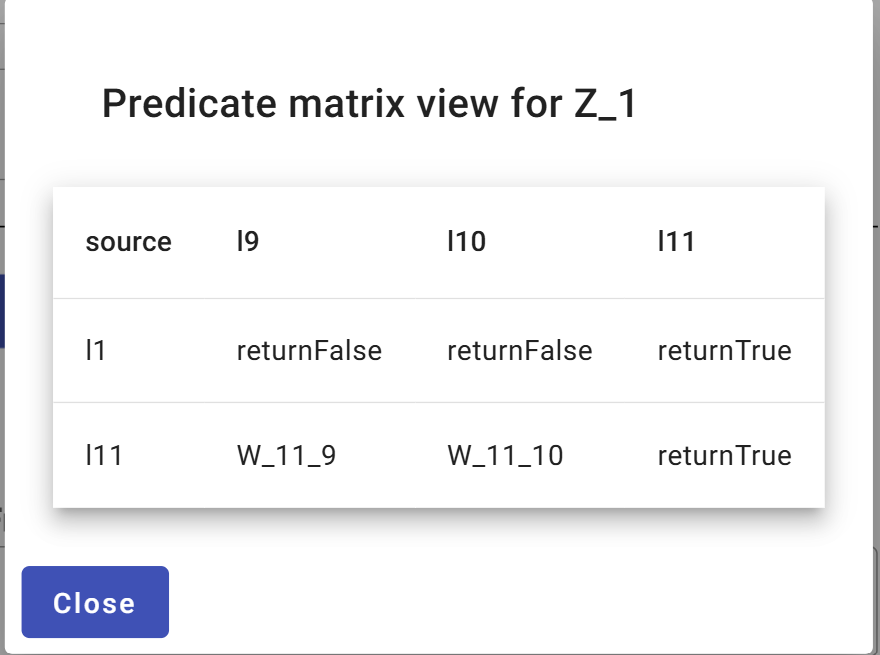
\includegraphics[width=0.52\linewidth]{../../4. applications/fuelGasEtc/images/matrix_1.png}}
		\captionsetup{width=0.8\textwidth}
		\caption*{\textbf{Figure~\ref{DIS-fig:onlinegn-matrix-z1}} -- Indexed matrix with predicates for transition $Z_1$ (CDU-2).}
	\end{figure}
	
	In this concrete example, the predicates reflect conditions of the type ``there is a request for LPG product from \textit{CDU-2}'' and ``there is a request for fuel gas product from \textit{CDU-2}''. In other words, transition $Z_1$ allows tokens to continue only when the corresponding requests/conditions described in the model are present. Analogously, indexed matrices are introduced for the remaining transitions, corresponding to the predicates described for the concrete process units and streams.
	
	The initial characteristics of the tokens are set according to the scenario from the article. In \textbf{Figure~\ref{DIS-fig:onlinegn-token-l1}} a token is shown in the input place $l_1$, which enters $Z_1$ (\textit{CDU-2}), together with its initial characteristic. This characteristic contains the necessary attributes for the simulation (e.g. type of request and quantities), so that during execution it can be clearly traced what the token ``carries'' and how it changes along the chain.
	
\begin{figure}[H]
	\centering
	\setlength{\fboxrule}{2pt}
	\setlength{\fboxsep}{0pt}
	\fbox{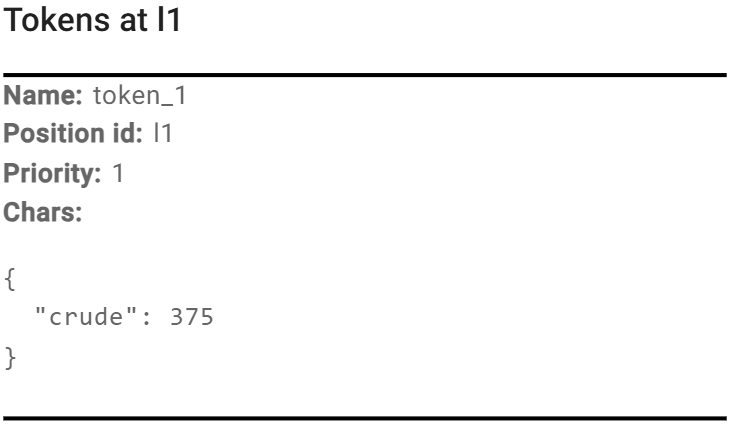
\includegraphics[width=0.52\linewidth]{../../4. applications/fuelGasEtc/images/token_1.png}}
	\captionsetup{width=0.8\textwidth}
	\caption*{\textbf{Figure~\ref{DIS-fig:onlinegn-token-l1}} -- Token in the input place $l_1$ with initial characteristic (example of input to $Z_1$).}
\end{figure}
	
	After successful execution of the simulation, the observed output characteristics coincide with the expected theoretical results. As a concrete illustration, at the output place $l_{53}$ (designated as \textit{``LPG TANKS''}) a token is obtained whose characteristic contains the amount of \textit{LPG} predicted by the model. This is shown in \textbf{Figure~\ref{DIS-fig:onlinegn-token-l53}}.
	
	\begin{figure}[H]
		\centering
		\setlength{\fboxrule}{2pt}
		\setlength{\fboxsep}{0pt}
		\fbox{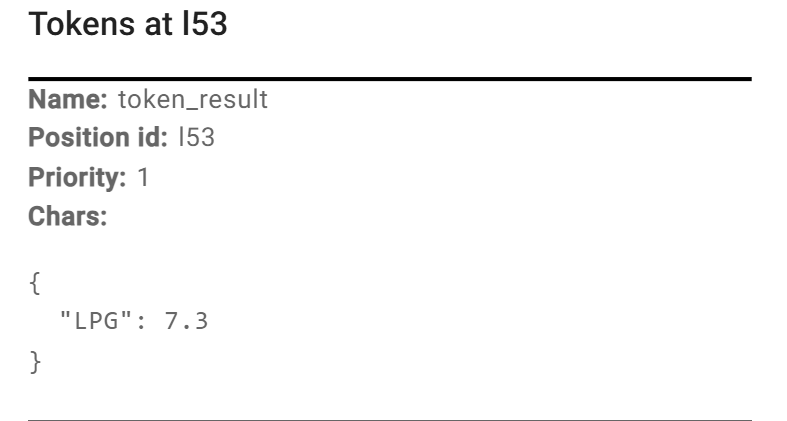
\includegraphics[width=0.52\linewidth]{../../4. applications/fuelGasEtc/images/token_2.png}}
		\captionsetup{width=0.8\textwidth}
		\caption*{\textbf{Figure~\ref{DIS-fig:onlinegn-token-l53}} -- Token in the output place $l_{53}$ (``LPG TANKS'') with characteristic after simulation.}
	\end{figure}
	
	In summary, the simulation results confirm that the specified predicates and initial characteristics work correctly and that the GN model adequately describes the production process under consideration. This gives grounds for accepting the model as validated with respect to the theoretical scenario and as usable for subsequent experiments and analyses.
	
	\subsubsection{Conclusions on the Model and the Simulation}
	
	\hspace*{2.5em}The production of gaseous products in a petroleum refinery (fuel gas, LPG, and propylene, including as raw material for polypropylene) is a complex parallel process in which correct reflection of the cause--effect relations is key; in GNs this is specified naturally through the predicates of the transition conditions. The present chapter presents a GN model and its software realization and simulation through \textit{OnlineGN}. Obtaining results corresponding to the expected behavior of the process confirms the correctness of the model and demonstrates the applicability of GNs in modeling and simulation of similar production chains.
	
	\subsection{Generalized-Net Model of the Production of Heavy Petroleum Products in a Petroleum Refinery}
	
	\hspace*{2.5em}Here, a GN model of the production of heavy petroleum products in a petroleum refinery and its simulation through \textit{OnlineGN} are considered. The construction of the model is described in detail in~\cite{DIS-Stratiev2023_2}.
	
	\subsubsection{Introduction to Generalized-Net Models for Petroleum Products in a Petroleum Refinery}
	
	\hspace*{2.5em}The dissertation considers that the production processes running in parallel in a petroleum refinery can be modeled and simulated through GNs~\cite{DIS-Z1}. In the present chapter, the focus is on the processing of heavy residual fractions and the production of heavy petroleum products. Heavy oil represents the residual petroleum fraction after atmospheric distillation~\cite{DIS-96}, with boiling temperature above 360~$^\circ$C and relative density above 0.933 (\textit{API} < 20)~\cite{DIS-97}. The aim is for the process to be modeled with the help of GNs and for the model to be simulated through \textit{OnlineGN}.
	
	\subsubsection{Processing Scheme for Production of Different Types of Heavy Fuel Oil and Road Pavement Bitumen in a Petroleum Refinery, Modeled through Generalized Nets}
	
	\hspace*{2.5em}The dissertation considers the production of three types of fuel oil with different sulfur content (\textit{Fuel oil} 0.5\%~\textit{S}, \textit{Fuel oil} 1.0\%~\textit{S}, \textit{Fuel oil} 2.5\%~\textit{S}) and the production of road bitumen in \textit{BU}, as shown in \textbf{Figure~\ref{DIS-fig1}}. The specifications and requirements for the fuel oils are presented in~\cite{DIS-Stratiev2023_2}. The vacuum fractions (\textit{VR}, \textit{SRVGO}) are obtained in \textit{VDU-1}/\textit{VDU-2} from the atmospheric residue (\textit{CDU})~\cite{DIS-103}.
	

\begin{figure}[H]
	\centering
	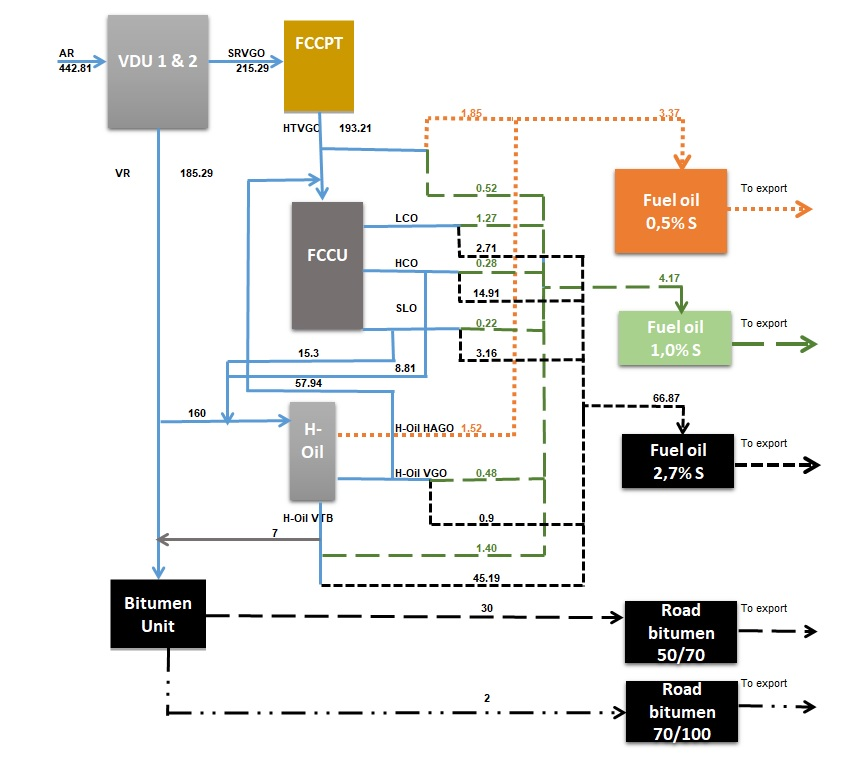
\includegraphics[scale=0.5]{../../4. applications/heavyOilProducts/images/Figure_1.jpg}%
	\caption*{\textbf{Figure~\ref{DIS-fig1}} -- Processing scheme for production of different grades of heavy fuel oil and road pavement 
		bitumen in a petroleum refinery to be modeled using generalized nets. The numbers in the diagram 
		are related to the quantity of the heavy oil streams in the dimension of t/h. Different colors are used 
		to differentiate the three grades of produced fuel oils: orange for fuel oil 0.5\% S, green for fuel oil 
		1.0\% S, and black for fuel oil 2.5\% S.}
\end{figure}
	
	\subsubsection{Results from Modeling the Production of Heavy Petroleum Products in a Petroleum Refinery with the Help of Generalized Nets}
	
	\hspace*{2.5em}The GN model (see \textbf{Figure~\ref{DIS-fig2}} in the dissertation) contains 8 transitions, 35 places, and 8 token types. The technological units \textit{VDU}, \textit{FCCPT}, \textit{FCCU}, \textit{H-Oil}, and \textit{BU}, as well as the outputs for 0.5\%~\textit{S}, 1.0\%~\textit{S}, and 2.5\%~\textit{S}, are modeled. At the initial moment, tokens $\alpha_0,\beta_0,\gamma_0,\delta_0,\epsilon_0,\zeta_0,\eta_0,\theta_0$ are placed respectively in places $l_1,l_9,l_{17},l_{26},l_{29},l_{31},l_{33},l_{35}$ with characteristics corresponding to \textit{AR}, \textit{SRVGO}, \textit{SRVR}, \textit{FCC} feedstock, bitumen feedstock, and final products. The logic of the process is specified through indexed matrices and predicates (e.g. $W_{5,2}, W_{5,3}, W_{5,4}$ for requests to \textit{VDU}), where during execution the tokens are merged and split depending on the truth values of the predicates and the specified quantities $q_i \in [0,Q_i]$.
	
\begin{figure}[H]
	\tiny
	\newcommand{\mytriangle}{\Large $\bigtriangledown$}
	%\begin{center}
	%   \begin{center}
		\setlength{\unitlength}{8.5pt} %10pt=4mm
		\linethickness{0.4pt}
		\begin{picture}(37, 71)
			%%% Transitions
			\put(3.0,71.0){\makebox(0,0)[cc]{$VDU$}}
			\put(3.0,69.0){\makebox(0,0)[bb]{\mytriangle}}
			\put(3.0,69.0){\line(0,-1){39}}
			\put(34.0,71){\makebox(0,0)[cc]{$BU$}}
			\put(34.0,69.0){\makebox(0,0)[bb]{\mytriangle}}
			\put(34.0,69.0){\line(0,-1){7}}
			\put(20.0,65.0){\makebox(0,0)[cc]{$H-Oil$}}
			\put(20.0,63.0){\makebox(0,0)[bb]{\mytriangle}}
			\put(20.0,63.0){\line(0,-1){17}}
			\put(34.0,57){\makebox(0,0)[cc]{$0.5\% S$}}
			\put(34.0,55.0){\makebox(0,0)[bb]{\mytriangle}}
			\put(34.0,55.0){\line(0,-1){7}}
			\put(20.0,39.0){\makebox(0,0)[cc]{$FCCU$}}
			\put(20.0,37.0){\makebox(0,0)[bb]{\mytriangle}}
			\put(20.0,37.0){\line(0,-1){19}}
			\put(34.0,39.0){\makebox(0,0)[cc]{$1.0\% S$}}
			\put(34.0,37.0){\makebox(0,0)[bb]{\mytriangle}}
			\put(34.0,37.0){\line(0,-1){15}}
			\put(10.0,37.0){\makebox(0,0)[cc]{$FCCPT$}}
			\put(10.0,35.0){\makebox(0,0)[bb]{\mytriangle}}
			\put(10.0,35.0){\line(0,-1){11}}
			\put(34.0,17.0){\makebox(0,0)[cc]{$2.5\% S$}}
			\put(34.0,15.0){\makebox(0,0)[bb]{\mytriangle}}
			\put(34.0,15.0){\line(0,-1){13}}
			%%% Input places
			\put(1.5,68.5){\makebox(0,0)[cc]{$l_{1}$}}
			\put(1.5,67.5){\circle{1.0}}
			\put(2.0,67.5){\vector(1,0){1.0}}
			%%% Output places
			\put(4.5,68.5){\makebox(0,0)[cc]{$l_{2}$}}
			\put(3.0,67.5){\vector(1,0){1.0}}
			\put(4.5,67.5){\circle{1.0}}
			\put(35.5,68.5){\makebox(0,0)[cc]{$l_{27}$}}
			\put(34.0,67.5){\vector(1,0){1.0}}
			\put(35.5,67.5){\circle{1.0}}
			\put(35.5,66.5){\makebox(0,0)[cc]{$l_{28}$}}
			\put(34.0,65.5){\vector(1,0){1.0}}
			\put(35.5,65.5){\circle{1.0}}
			\put(35.5,64.5){\makebox(0,0)[cc]{$l_{29}$}}
			\put(34.0,63.5){\vector(1,0){1.0}}
			\put(35.5,63.5){\circle{1.0}}
			\put(4.5,62.5){\makebox(0,0)[cc]{$l_{3}$}}
			\put(3.0,61.5){\vector(1,0){1.0}}
			\put(4.5,61.5){\circle{1.0}}
			\put(21.5,62.5){\makebox(0,0)[cc]{$l_{10}$}}
			\put(20.0,61.5){\vector(1,0){1.0}}
			\put(21.5,61.5){\circle{1.0}}
			\put(21.5,60.5){\makebox(0,0)[cc]{$l_{11}$}}
			\put(20.0,59.5){\vector(1,0){1.0}}
			\put(21.5,59.5){\circle{1.0}}
			\put(21.5,58.5){\makebox(0,0)[cc]{$l_{12}$}}
			\put(20.0,57.5){\vector(1,0){1.0}}
			\put(21.5,57.5){\circle{1.0}}
			\put(21.5,56.5){\makebox(0,0)[cc]{$l_{13}$}}
			\put(20.0,55.5){\vector(1,0){1.0}}
			\put(21.5,55.5){\circle{1.0}}
			\put(21.5,54.5){\makebox(0,0)[cc]{$l_{14}$}}
			\put(20.0,53.5){\vector(1,0){1.0}}
			\put(21.5,53.5){\circle{1.0}}
			\put(35.5,54.5){\makebox(0,0)[cc]{$l_{30}$}}
			\put(34.0,53.5){\vector(1,0){1.0}}
			\put(35.5,53.5){\circle{1.0}}
			\put(21.5,52.5){\makebox(0,0)[cc]{$l_{15}$}}
			\put(20.0,51.5){\vector(1,0){1.0}}
			\put(21.5,51.5){\circle{1.0}}
			\put(21.5,50.5){\makebox(0,0)[cc]{$l_{16}$}}
			\put(20.0,49.5){\vector(1,0){1.0}}
			\put(21.5,49.5){\circle{1.0}}
			\put(35.5,50.5){\makebox(0,0)[cc]{$l_{31}$}}
			\put(34.0,49.5){\vector(1,0){1.0}}
			\put(35.5,49.5){\circle{1.0}}
			\put(21.5,48.5){\makebox(0,0)[cc]{$l_{17}$}}
			\put(20.0,47.5){\vector(1,0){1.0}}
			\put(21.5,47.5){\circle{1.0}}
			\put(21.5,36.5){\makebox(0,0)[cc]{$l_{18}$}}
			\put(20.0,35.5){\vector(1,0){1.0}}
			\put(21.5,35.5){\circle{1.0}}
			\put(4.5,34.5){\makebox(0,0)[cc]{$l_{4}$}}
			\put(3.0,33.5){\vector(1,0){1.0}}
			\put(4.5,33.5){\circle{1.0}}
			\put(11.5,34.5){\makebox(0,0)[cc]{$l_{6}$}}
			\put(10.0,33.5){\vector(1,0){1.0}}
			\put(11.5,33.5){\circle{1.0}}
			\put(21.5,34.5){\makebox(0,0)[cc]{$l_{19}$}}
			\put(20.0,33.5){\vector(1,0){1.0}}
			\put(21.5,33.5){\circle{1.0}}
			\put(4.5,32.5){\makebox(0,0)[cc]{$l_{5}$}}
			\put(3.0,31.5){\vector(1,0){1.0}}
			\put(4.5,31.5){\circle{1.0}}
			\put(21.5,32.5){\makebox(0,0)[cc]{$l_{20}$}}
			\put(20.0,31.5){\vector(1,0){1.0}}
			\put(21.5,31.5){\circle{1.0}}
			\put(35.5,32.5){\makebox(0,0)[cc]{$l_{32}$}}
			\put(34.0,31.5){\vector(1,0){1.0}}
			\put(35.5,31.5){\circle{1.0}}
			\put(11.5,30.5){\makebox(0,0)[cc]{$l_{7}$}}
			\put(10.0,29.5){\vector(1,0){1.0}}
			\put(11.5,29.5){\circle{1.0}}
			\put(21.5,30.5){\makebox(0,0)[cc]{$l_{21}$}}
			\put(20.0,29.5){\vector(1,0){1.0}}
			\put(21.5,29.5){\circle{1.0}}
			\put(11.5,28.5){\makebox(0,0)[cc]{$l_{8}$}}
			\put(10.0,27.5){\vector(1,0){1.0}}
			\put(11.5,27.5){\circle{1.0}}
			\put(21.5,28.5){\makebox(0,0)[cc]{$l_{22}$}}
			\put(20.0,27.5){\vector(1,0){1.0}}
			\put(21.5,27.5){\circle{1.0}}
			\put(11.5,26.5){\makebox(0,0)[cc]{$l_{9}$}}
			\put(10.0,25.5){\vector(1,0){1.0}}
			\put(11.5,25.5){\circle{1.0}}
			\put(21.5,26.5){\makebox(0,0)[cc]{$l_{23}$}}
			\put(20.0,25.5){\vector(1,0){1.0}}
			\put(21.5,25.5){\circle{1.0}}
			\put(21.5,24.5){\makebox(0,0)[cc]{$l_{24}$}}
			\put(20.0,23.5){\vector(1,0){1.0}}
			\put(21.5,23.5){\circle{1.0}}
			\put(35.5,24.5){\makebox(0,0)[cc]{$l_{33}$}}
			\put(34.0,23.5){\vector(1,0){1.0}}
			\put(35.5,23.5){\circle{1.0}}
			\put(21.5,22.5){\makebox(0,0)[cc]{$l_{25}$}}
			\put(20.0,21.5){\vector(1,0){1.0}}
			\put(21.5,21.5){\circle{1.0}}
			\put(21.5,20.5){\makebox(0,0)[cc]{$l_{26}$}}
			\put(20.0,19.5){\vector(1,0){1.0}}
			\put(21.5,19.5){\circle{1.0}}
			\put(35.5,10.5){\makebox(0,0)[cc]{$l_{34}$}}
			\put(34.0,9.5){\vector(1,0){1.0}}
			\put(35.5,9.5){\circle{1.0}}
			\put(35.5,4.5){\makebox(0,0)[cc]{$l_{35}$}}
			\put(34.0,3.5){\vector(1,0){1.0}}
			\put(35.5,3.5){\circle{1.0}}
			%%% Vertical paths
			\put(30.5,65.5){\line(0,-1){4}}
			\put(31.5,63.5){\line(0,-1){3}}
			\put(36.5,63.5){\line(0,-1){3}}
			\put(31.5,59.5){\line(0,-1){6}}
			\put(30.5,57.5){\line(0,-1){22}}
			\put(29.5,55.5){\line(0,-1){22}}
			\put(26.5,53.5){\line(0,-1){40}}
			\put(15.5,51.5){\line(0,-1){8}}
			\put(25.5,51.5){\line(0,-1){40}}
			\put(28.5,51.5){\line(0,-1){10}}
			\put(16.5,49.5){\line(0,-1){9}}
			\put(23.5,49.5){\line(0,-1){10}}
			\put(31.5,49.5){\line(0,-1){3}}
			\put(36.5,49.5){\line(0,-1){3}}
			\put(17.5,47.5){\line(0,-1){3}}
			\put(22.5,47.5){\line(0,-1){3}}
			\put(24.5,43.5){\line(0,-1){10}}
			\put(12.5,41.5){\line(0,-1){8}}
			\put(22.5,40.5){\line(0,-1){5}}
			\put(17.5,39.5){\line(0,-1){4}}
			\put(0.5,31.5){\line(0,-1){3}}
			\put(5.5,31.5){\line(0,-1){3}}
			\put(13.5,27.5){\line(0,-1){12}}
			\put(7.5,25.5){\line(0,-1){3}}
			\put(12.5,25.5){\line(0,-1){3}}
			\put(24.5,25.5){\line(0,-1){16}}
			\put(29.5,25.5){\line(0,-1){10}}
			\put(23.5,23.5){\line(0,-1){16}}
			\put(31.5,23.5){\line(0,-1){3}}
			\put(36.5,23.5){\line(0,-1){3}}
			\put(30.5,21.5){\line(0,-1){16}}
			\put(17.5,19.5){\line(0,-1){3}}
			\put(22.5,19.5){\line(0,-1){3}}
			\put(31.5,3.5){\line(0,-1){3}}
			\put(36.5,3.5){\line(0,-1){3}}
			%%% Horizontal paths
			\put(30.5,65.5){\vector(1,0){3.5}}
			\put(31.5,63.5){\vector(1,0){2.5}}
			\put(31.5,60.5){\line(1,0){5}}
			\put(31.5,53.5){\vector(1,0){2.5}}
			\put(15.5,51.5){\vector(1,0){4.5}}
			\put(28.5,51.5){\vector(1,0){5.5}}
			\put(16.5,49.5){\vector(1,0){3.5}}
			\put(31.5,49.5){\vector(1,0){2.5}}
			\put(17.5,47.5){\vector(1,0){2.5}}
			\put(31.5,46.5){\line(1,0){5}}
			\put(17.5,44.5){\line(1,0){5}}
			\put(15.5,43.5){\line(1,0){9}}
			\put(12.5,41.5){\line(1,0){16}}
			\put(16.5,40.5){\line(1,0){6}}
			\put(17.5,39.5){\line(1,0){6}}
			\put(17.5,35.5){\vector(1,0){2.5}}
			\put(30.5,35.5){\vector(1,0){3.5}}
			\put(29.5,33.5){\vector(1,0){4.5}}
			\put(0.5,31.5){\vector(1,0){2.5}}
			\put(0.5,28.5){\line(1,0){5}}
			\put(7.5,25.5){\vector(1,0){2.5}}
			\put(29.5,25.5){\vector(1,0){4.5}}
			\put(31.5,23.5){\vector(1,0){2.5}}
			\put(7.5,22.5){\line(1,0){5}}
			\put(31.5,20.5){\line(1,0){5}}
			\put(17.5,19.5){\vector(1,0){2.5}}
			\put(17.5,16.5){\line(1,0){5}}
			\put(13.5,15.5){\line(1,0){16}}
			\put(26.5,13.5){\vector(1,0){7.5}}
			\put(25.5,11.5){\vector(1,0){8.5}}
			\put(24.5,9.5){\vector(1,0){9.5}}
			\put(23.5,7.5){\vector(1,0){10.5}}
			\put(30.5,5.5){\vector(1,0){3.5}}
			\put(31.5,3.5){\vector(1,0){2.5}}
			\put(31.5,0.5){\line(1,0){5}}
			%%% Horizontal paths from output places
			\put(5.0,67.5){\vector(1,0){29}}
			\put(5.0,61.5){\vector(1,0){15}}
			\put(22.0,61.5){\line(1,0){8.5}}
			\put(22.0,59.5){\line(1,0){9.5}}
			\put(22.0,57.5){\line(1,0){8.5}}
			\put(22.0,55.5){\line(1,0){7.5}}
			\put(22.0,53.5){\line(1,0){4.5}}
			\put(22.0,51.5){\line(1,0){3.5}}
			\put(22.0,49.5){\line(1,0){1.5}}
			\put(5.0,33.5){\vector(1,0){5}}
			\put(22.0,33.5){\line(1,0){2.5}}
			\put(22.0,31.5){\vector(1,0){12}}
			\put(12.0,29.5){\vector(1,0){8}}
			\put(22.0,29.5){\vector(1,0){12}}
			\put(12.0,27.5){\line(1,0){1.5}}
			\put(22.0,27.5){\vector(1,0){12}}
			\put(22.0,25.5){\line(1,0){2.5}}
			\put(22.0,23.5){\line(1,0){1.5}}
			\put(22.0,21.5){\line(1,0){8.5}}
			%%% Corners
			\put(36.0,63.5){\line(1,0){0.5}}
			\put(36.0,49.5){\line(1,0){0.5}}
			\put(22.0,47.5){\line(1,0){0.5}}
			\put(22.0,35.5){\line(1,0){0.5}}
			\put(12.0,33.5){\line(1,0){0.5}}
			\put(5.0,31.5){\line(1,0){0.5}}
			\put(12.0,25.5){\line(1,0){0.5}}
			\put(36.0,23.5){\line(1,0){0.5}}
			\put(22.0,19.5){\line(1,0){0.5}}
			\put(36.0,3.5){\line(1,0){0.5}}
		\end{picture}
		\caption*{\textbf{Figure~\ref{DIS-fig2}} -- A GN model of the manufacturing of heavy oil products in ``LUKOIL Neftohim Burgas'' refinery.}
		% \end{center}
\end{figure}
	
	\subsubsection{Simulation of the Model with \textit{OnlineGN}}
	
	\hspace*{2.5em}The dissertation considers implementation and execution of the GN model in \textit{OnlineGN} for the purpose of verification and derivation of quantitative results. \textbf{Figure~\ref{DIS-fig:model}} shows the GN scheme integrated in the simulator. For the considered scenario, the initial token in place $l_1$ is atmospheric residue (\textit{AR}) with characteristic value 442.81, and the requests to the subsequent units are specified through the characteristic functions (\textit{code}) and the indexed matrices of the transitions. The results are derived from the characteristics of the tokens in the output places (e.g. $l_{32}$ for 1.0~mass.\% \textit{S} and $l_{34}$ for 2.5~mass.\% \textit{S}).
	
\begin{figure}[H]
	\centering
	\setlength{\fboxrule}{2pt}
	\setlength{\fboxsep}{0pt}
	\fbox{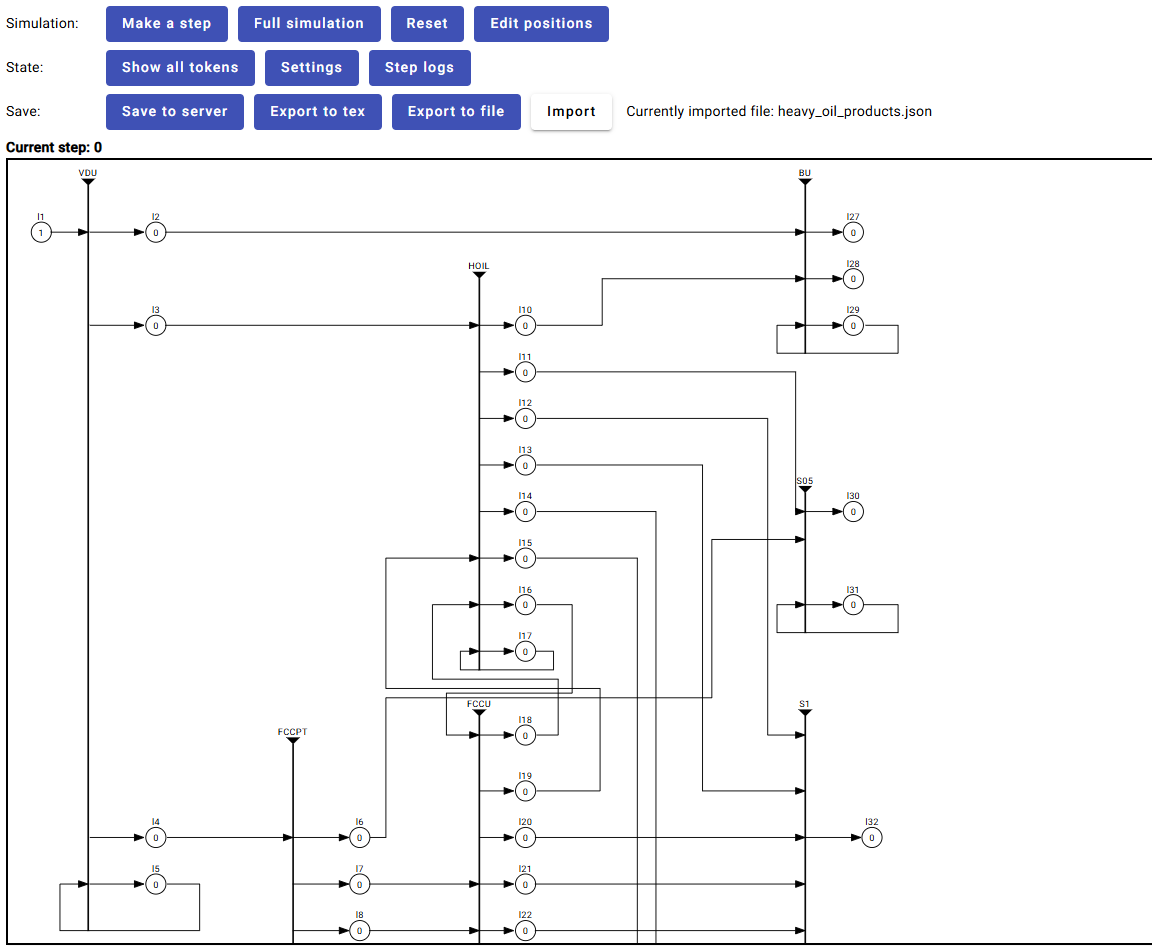
\includegraphics[width=0.95\linewidth]{../../4. applications/heavyOilProducts/images/model5.png}}
	\captionsetup{width=0.9\textwidth}
	\caption*{\textbf{Figure~\ref{DIS-fig:model}} -- Generalized net (GN) model of the heavy oil products processing chain in the refinery.}
\end{figure}


\begin{figure}[H]
	\centering
	\setlength{\fboxrule}{2pt}
	\setlength{\fboxsep}{0pt}
	\fbox{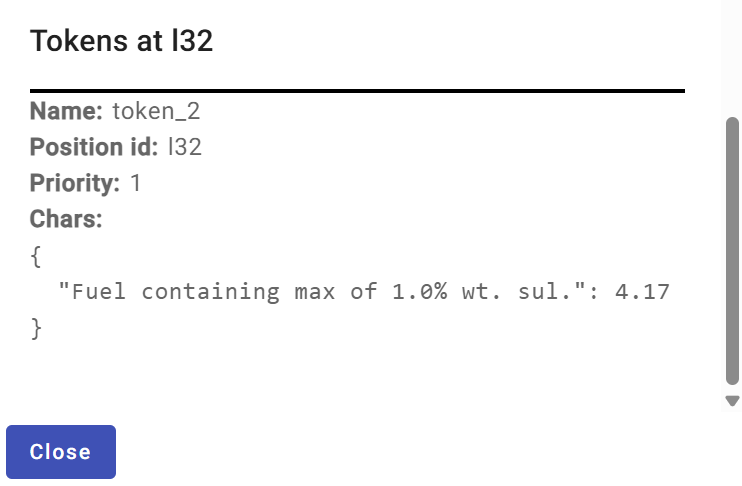
\includegraphics[width=0.6\linewidth]{../../4. applications/heavyOilProducts/images/1r.png}}
	\captionsetup{width=0.7\textwidth}
	\caption*{\textbf{Figure~\ref{DIS-fig:res1}} -- Obtained quantity of fuel oil with a maximum of 1.0 wt.\% sulfur (place $l_{32}$).}
\end{figure}
	
	\subsubsection{Results for the Model}
	
	\hspace*{2.5em}As can be seen in \textbf{Figure~\ref{DIS-fig1}}, the production of the three classes of heavy fuel oil and of the classes of road pavement bitumen is a complex parallel process involving \textit{VDU}, \textit{FCCPT}, \textit{FCCU}, \textit{H-Oil}, and \textit{BU}, within which refined heavy petroleum products and final product streams are obtained.
	
	\subsubsection{Conclusions}
	
	\hspace*{2.5em}The obtained results show that the processes of production of different classes of heavy petroleum products in a refinery can be successfully modeled through GNs, while the parallel nature and the cause--effect dependencies are represented naturally. The simulation carried out through \textbf{\textit{OnlineGN}} leads to results corresponding to the expected behavior of the system, which serves as verification of the correctness of the model and confirms the applicability of GNs in modeling and simulation of production processes in a petroleum refinery.
	
	\clearpage
	\phantomsection
	\addcontentsline{toc}{section}{Conclusion}
	
	\section*{Conclusion}
	
	\hspace*{2.5em}In the present dissertation, the main goal set was achieved -- the development of a new simulator for GNs functioning in an online environment, which substantially facilitates and accelerates work with GNs. The implemented solution supports key activities such as model creation, subsequent editing (including changes of functions and visualization), and efficient sharing of nets. During the development, modern and widely established technologies were used, aligned with the requirements for reliability, extensibility, and usability in a web environment.
	
	Alongside the software result, the dissertation also produced new contributions related to the theory and application of GNs. New algorithms were developed, aimed at supporting the modeling and presentation of GNs. First, an algorithm was proposed for automatic drawing of a GN from its description, which shortens the time needed to obtain a correct and clear visualization and limits the need for manual corrections. Second, an algorithm was developed for exporting the net in \textit{TeX} format, so that after edits and visual adjustments in the simulator, the model can be directly included in scientific publications and other academic materials.
	
	In addition, new GN models were created in different application areas, which demonstrate the expressive power of the apparatus and validate the capabilities of the developed simulator. Among them are models related to the representation of finite automata, a model of a mathematical game, as well as models of industrial processes, including scenarios related to the production of gas and petroleum products. All proposed models were implemented and studied through simulations with the simulator developed in the dissertation, which provides practical verification of the functionality and applicability of the system.
	
	\clearpage
	\phantomsection
	\addtocontents{toc}{\vspace{-1.0em}}
	\addcontentsline{toc}{section}{Author's Reference}
	\section*{Author's Reference}
	
	\addcontentsline{toc}{subsection}{Reference of the Contributions in the Dissertation}
	\subsection*{Reference of the Contributions in the Dissertation}
	
	\addcontentsline{toc}{subsubsection}{Scientific Contributions}
	\subsubsection*{Scientific Contributions}
	
	The following scientific contributions have been achieved in the present dissertation:
	
	\begin{enumerate}[label=\arabic*., leftmargin=*]
		\item \textbf{Algorithms for automation and visualization of Generalized Nets (GNs):}
		\begin{itemize}
			\item An algorithm for automated drawing of GNs on the basis of their abstract description has been developed, eliminating the need for manual specification of coordinates.
			\item An algorithm has been created for transforming vector images (\textit{SVG}) of GNs into \textit{TeX} format through identification of graphical primitives and coordinate transformation.
		\end{itemize}
		
		\item \textbf{Parallel solution of an exponential problem (Towers of Hanoi):}
		\begin{itemize}
			\item A new parallel variant of the Towers of Hanoi problem has been formalized, allowing simultaneous movement of up to $k$ rings.
			\item A theorem has been proved for the minimum number of parallel steps, $H(n,k) = 2^{\bigl\lceil \textstyle \frac{n}{k} \bigr\rceil} - 1$, and a constructive algorithm has been implemented for solving the problem.
		\end{itemize}
		
		\item \textbf{Generalized-net modeling and simulation of the parallel exponential Towers of Hanoi problem:}
		\begin{itemize}
			\item An original GN model of the parallel Towers of Hanoi has been created, using $\rho$-tokens for the objects and $\chi$-tokens for the resources.
			\item The applicability of the formalism has been demonstrated through simulations in the \textit{OnlineGN} environment, showing effective management of concurrent processes and logical constraints.
		\end{itemize}
	\end{enumerate}
	
	\addcontentsline{toc}{subsubsection}{Scientific--Applied Contributions}
	\subsubsection*{Scientific--Applied Contributions}
	
	The following results have been achieved from a scientific--applied point of view:
	
	\begin{enumerate}[label=\arabic*., leftmargin=*]
		\item \textbf{Design, implementation, and application of the software system \textit{OnlineGN}:}
		\begin{itemize}
			\item An innovative web-based platform has been developed for modeling, simulation, and visualization of GNs, offering a centralized environment without the need for local installation.
			\item A convenient and interactive interface has been developed for changing each GN component in the simulator, as well as for tracking details of the execution of the net.
			\item Functionality has been implemented for export from \textit{SVG} to \textit{TeX}, which optimizes the preparation of graphical materials for academic publications.
		\end{itemize}
		
		\item \textbf{A new method for representation of finite automata through GNs:}
		\begin{itemize}
			\item A methodology has been developed for describing deterministic and nondeterministic finite automata through GNs, allowing the capture of parallel computation paths.
		\end{itemize}
		
		\item \textbf{Modeling of existing processes in a petroleum refinery through GNs:}
		\begin{itemize}
			\item GN models have been developed for real technological processes in a petroleum refinery, including the production of gas, polymeric, and heavy petroleum products.
		\end{itemize}
		
		\item \textbf{Verification of the new GN models through \textit{OnlineGN}:}
		\begin{itemize}
			\item All newly created models in the dissertation have been verified through simulations in \textit{OnlineGN}, which simultaneously verifies both the correctness of the models and the capabilities of the system.
		\end{itemize}
	\end{enumerate}
	
	\clearpage
	\phantomsection
	\addcontentsline{toc}{section}{Publications Related to the Dissertation}
	\section*{Publications Related to the Dissertation}
	
	\begin{enumerate}[label=\arabic*.]
		
		\item Dimitriev, A.; Terziev, G.
		\newblock \emph{Automating Creativity: Enhancing Generalized Nets with Algorithmic Drawing}.
		\newblock In: \emph{Proceedings of the 22nd International Workshop on Intuitionistic Fuzzy Sets and Generalized Nets}, Warsaw, Poland, October 18, 2024 (in press).
		
		\item Dimitriev, A.
		\newblock \emph{Representing Finite-State Automata with Generalized Nets: Simulation via OnlineGN}.
		\newblock \emph{Proceedings of the Jangjeon Mathematical Society}, vol.~29, no.~1, pp.~156--167, Jan.~2026.
		\newblock doi: \url{ https://doi.org/10.17777/pjms.2026.29.1.011}.
		
		\item Dimitriev, A.; Atanassov, K.; Angelova, N.
		\newblock \emph{Parallel Towers of Hanoi via Generalized Nets: Simulated with OnlineGN}.
		\newblock \emph{Software}, vol.~4, no.~4, art.~23, 2025.
		\newblock doi: \url{ https://doi.org/10.3390/software4040023}.
		
		\item Stratiev, D. D.; Dimitriev, A.; Stratiev, D.; Atanassov, K.
		\newblock \emph{Modeling the Production Process of Fuel Gas, LPG, Propylene, and Polypropylene in a Petroleum Refinery Using Generalized Nets}.
		\newblock \emph{Mathematics}, 2023, \textbf{11}, 3800.
		\newblock doi: \url{ https://doi.org/10.3390/math11173800}.
		
		\item Stratiev, D. D.; Dimitriev, A.; Stratiev, D.; Atanassov, K.
		\newblock \emph{Generalized Net Model of Heavy Oil Products' Manufacturing in Petroleum Refinery}.
		\newblock \emph{Mathematics}, 2023, \textbf{11}, 4753.
		\newblock doi: \url{ https://doi.org/10.3390/math11234753}.
		
	\end{enumerate}